\chapter{DỮ LIỆU VÀ PHƯƠNG PHÁP NGHIÊN CỨU}

Chương này trình bày thiết kế nghiên cứu và cách thức triển khai thực nghiệm trên hai bộ dữ liệu tín dụng. Trước hết, chương xác định phạm vi của bài toán, mô tả nguồn dữ liệu và giới thiệu các công nghệ được sử dụng để xây dựng hệ thống. Tiếp theo, quy trình nghiên cứu được trình bày theo các bước từ phân tích khám phá, làm sạch và tiền xử lý dữ liệu đến xây dựng đặc trưng, kiểm soát rò rỉ thông tin và xử lý mất cân bằng lớp. Phần cuối của chương mô tả phương pháp chia mẫu, huấn luyện, hiệu chỉnh, triển khai và giám sát mô hình. Cách tổ chức này nhằm bảo đảm sự liên kết giữa cơ sở lý thuyết ở Chương 2 với quy trình tạo ra các kết quả thực nghiệm được phân tích ở Chương 4.

\section{Định hướng và phạm vi thực nghiệm}

Nguồn dữ liệu gồm hai bộ dữ liệu chứa thông tin đã được mã hóa về các khoản vay tại ngân hàng thương mại thuộc phạm vi nghiên cứu. Bộ dữ liệu A, \path{Data_credit_rating_VN.xlsx}, gồm 27.001 quan sát và 21 biến ban đầu; biến đích \mbox{\texttt{NHOMNOMOI}} nhận giá trị từ 1 đến 5, tương ứng với năm nhóm nợ. Bộ dữ liệu B được trích xuất từ hai kỳ báo cáo liên tiếp của cùng một tổ chức tín dụng: \texttt{Thông tin tín dụng 20260430.xlsx} (100.617 hợp đồng và 41 cột thô, dùng để huấn luyện và kiểm định nội bộ) và \texttt{Thông tin tín dụng 20260507.xlsx} (100.274 hợp đồng và 33 cột thô, dùng làm \emph{tập kiểm tra độc lập}, hoàn toàn tách biệt khỏi quá trình huấn luyện). Biến đích \texttt{Nhóm nợ tự phân loại} cũng nhận giá trị từ 1 đến 5. Do tập dữ liệu kỳ 20260507 chỉ chứa 33 trong tổng số 41 cột của kỳ 20260430, tập đặc trưng của bộ B chỉ được xây dựng từ các cột hiện diện ở cả hai kỳ. Ràng buộc này bảo đảm rằng mô hình được huấn luyện trên kỳ 20260430 có thể áp dụng cho kỳ 20260507 (Mục \ref{sec:pool-a}).

Phạm vi thực nghiệm của luận văn gồm hai bài toán có mục tiêu khác nhau. Bài toán thứ nhất phân loại trạng thái hiện tại của khoản vay vào một trong năm nhóm nợ trên hai bộ dữ liệu A và B. Bài toán thứ hai dự báo khả năng khoản vay chuyển sang nhóm nợ có mức rủi ro cao hơn trong tháng kế tiếp, được xây dựng bằng cách ghép hai kỳ báo cáo liên tiếp của bộ B. Bài toán thứ hai hướng trực tiếp tới mục tiêu hỗ trợ cảnh báo sớm, trong khi bài toán thứ nhất được sử dụng để đối sánh phương pháp mô hình hóa, đánh giá vai trò của các nhóm đặc trưng và kiểm tra khả năng tổng quát hóa ngoài mẫu.

Nếu có dữ liệu bảng theo thời gian, nhãn chuyển nhóm cần được định nghĩa:
\[
Y_{i,t}^{(h)}
=
\begin{cases}
1, & G_{i,t+h}>G_{i,t},\\
0, & G_{i,t+h}\leq G_{i,t},
\end{cases}
\]
trong đó $i$ biểu thị khoản vay hoặc khách hàng; $t$ là thời điểm quan sát; $h$ là khoảng dự báo; $G_{i,t}\in\{1,2,3,4,5\}$ là nhóm nợ tại thời điểm $t$; và $Y_{i,t}^{(h)}=1$ biểu thị sự chuyển dịch sang nhóm có mức rủi ro cao hơn trong khoảng $h$. Trong thực nghiệm trên bộ B, luận văn sử dụng hai kỳ báo cáo liên tiếp và xác định $h=1$ tháng. Toàn bộ đặc trưng đầu vào được lấy tại thời điểm $t$, còn trạng thái tại $t+h$ chỉ được sử dụng để xây dựng nhãn, qua đó hạn chế nguy cơ rò rỉ thông tin từ tương lai.

\section{Quy trình nghiên cứu tổng thể}
\label{sec:pipeline-overview}

Quy trình thực nghiệm được tổ chức thành bảy bước tuần tự, thể hiện tại Hình \ref{fig:experimental-pipeline}: (1) thu thập dữ liệu gốc; (2) phân tích khám phá và làm sạch dữ liệu; (3) tiền xử lý và lựa chọn biến, bao gồm tính WOE/IV, mã hóa và chuẩn hóa; (4) phân chia tập huấn luyện--kiểm định và xử lý mất cân bằng lớp; (5) huấn luyện mô hình; (6) đánh giá hiệu quả và giải thích kết quả; và (7) rút ra kết luận cùng khuyến nghị ứng dụng. Cấu trúc này góp phần hạn chế ảnh hưởng của dữ liệu kiểm định đối với quá trình huấn luyện và phù hợp với nguyên tắc đánh giá ngoài mẫu trong học máy \cite{bishop2006pattern,lessmann2015benchmarking}.

\begin{figure}[H]
\centering
\begin{tabular}{c}
\fbox{\parbox[c][1.5cm][c]{9.6cm}{\centering \textbf{1. Thu thập dữ liệu}\\\footnotesize Khoản vay, khách hàng, lịch sử trả nợ}}\\[1mm]
$\Downarrow$\\[1mm]
\fbox{\parbox[c][1.5cm][c]{9.6cm}{\centering \textbf{2. EDA \& làm sạch dữ liệu}\\\footnotesize Giá trị thiếu, ngoại lệ, phân phối}}\\[1mm]
$\Downarrow$\\[1mm]
\fbox{\parbox[c][1.5cm][c]{9.6cm}{\centering \textbf{3. Tiền xử lý \& chọn biến}\\\footnotesize WOE/IV, mã hóa, chuẩn hóa}}\\[1mm]
$\Downarrow$\\[1mm]
\fbox{\parbox[c][1.5cm][c]{9.6cm}{\centering \textbf{4. Chia dữ liệu \& cân bằng lớp}\\\footnotesize Train/test, SMOTE, class weight}}\\[1mm]
$\Downarrow$\\[1mm]
\fbox{\parbox[c][1.5cm][c]{9.6cm}{\centering \textbf{5. Huấn luyện mô hình}\\\footnotesize LR, RF, XGBoost, LightGBM\ldots}}\\[1mm]
$\Downarrow$\\[1mm]
\fbox{\parbox[c][1.5cm][c]{9.6cm}{\centering \textbf{6. Đánh giá \& giải thích}\\\footnotesize F1, AUC, ma trận nhầm lẫn, SHAP}}\\[1mm]
$\Downarrow$\\[1mm]
\fbox{\parbox[c][1.5cm][c]{9.6cm}{\centering \textbf{7. Kết luận \& ứng dụng}\\\footnotesize Cảnh báo sớm, khuyến nghị}}\\
\end{tabular}
\caption{Pipeline nghiên cứu tổng thể — từ thu thập dữ liệu tới kết luận và ứng dụng}
\label{fig:experimental-pipeline}
\end{figure}

\section{Công nghệ và môi trường triển khai}
\label{sec:technologies}

Toàn bộ quy trình thực nghiệm và ứng dụng minh họa được xây dựng bằng Python 3.11. Ngôn ngữ này được lựa chọn nhờ hệ sinh thái thư viện tương đối hoàn chỉnh cho xử lý dữ liệu, học máy, giải thích mô hình và phát triển ứng dụng tương tác. Các công nghệ chính được tổng hợp tại Bảng \ref{tab:technologies}. Danh sách này được xác định từ tệp \texttt{requirements.txt} và các mô-đun được sử dụng trực tiếp trong mã nguồn của nghiên cứu.

\begin{table}[H]
\centering
\caption{Các công nghệ chính được sử dụng trong nghiên cứu}
\label{tab:technologies}
\begin{tabular}{|p{3.4cm}|p{4.0cm}|p{6.3cm}|}
\hline
\textbf{Công nghệ} & \textbf{Vai trò} & \textbf{Nội dung sử dụng trong luận văn}\\
\hline
Python 3.11 & Ngôn ngữ lập trình & Tổ chức quy trình xử lý dữ liệu, huấn luyện, đánh giá, lưu trữ và phục vụ mô hình.\\
\hline
pandas, NumPy & Xử lý và tính toán dữ liệu & Đọc dữ liệu Excel, biến đổi bảng dữ liệu, xử lý giá trị thiếu, xây dựng đặc trưng và thực hiện các phép tính ma trận.\\
\hline
scikit-learn & Học máy và đánh giá & Xây dựng Logistic Regression, Decision Tree, Random Forest, quy trình tiền xử lý, chia mẫu và tính các chỉ tiêu đánh giá.\\
\hline
imbalanced-learn & Xử lý mất cân bằng lớp & Xây dựng quy trình có SMOTE, BorderlineSMOTE, ADASYN, SMOTETomek và lấy mẫu dưới ngẫu nhiên.\\
\hline
XGBoost, LightGBM, CatBoost & Mô hình boosting & Huấn luyện và đối sánh ba họ mô hình tăng cường dựa trên cây quyết định.\\
\hline
SHAP & Giải thích mô hình & Ước lượng đóng góp của đặc trưng ở phạm vi toàn cục, theo nhóm nghiệp vụ và đối với từng quan sát.\\
\hline
Plotly, Matplotlib & Trực quan hóa & Biểu diễn phân bố dữ liệu, ma trận nhầm lẫn, đường cong hiệu năng và mức độ quan trọng của đặc trưng.\\
\hline
Streamlit & Ứng dụng minh họa & Xây dựng giao diện phân tích khám phá, huấn luyện, chấm điểm, dự báo và so sánh mô hình.\\
\hline
OpenPyXL, Pickle & Trao đổi và lưu trữ & Đọc--ghi tệp Excel và tuần tự hóa mô hình đã huấn luyện để tái sử dụng trong ứng dụng.\\
\hline
\end{tabular}
\end{table}

Về kiến trúc, lớp dữ liệu được quản lý bằng pandas và NumPy; lớp mô hình hóa được triển khai trên scikit-learn, imbalanced-learn cùng ba thư viện boosting; lớp giải thích và trực quan hóa sử dụng SHAP, Plotly và Matplotlib; trong khi Streamlit đảm nhiệm lớp giao diện. Cách phân tách này giúp các bước tiền xử lý, huấn luyện và đánh giá được tái sử dụng thống nhất giữa các chức năng của ứng dụng.

\section{Bước 1: Thu thập dữ liệu}
\label{sec:step1-collect}

Bước đầu tiên của quy trình gồm thu thập và kiểm tra hai tệp dữ liệu gốc, xác định biến đích và khảo sát sơ bộ phân bố nhóm nợ trước khi thực hiện các bước xử lý tiếp theo.

\subsection{Bộ dữ liệu A: Data\_credit\_rating\_VN}
\label{sec:dataset-a-structure}

Bộ dữ liệu A gồm 27.001 hợp đồng vay và không có bản ghi thiếu dữ liệu tại biến đích \mbox{\texttt{NHOMNOMOI}}. Theo Bảng \ref{tab:dataset-a-distribution}, nhóm 1 chiếm 77,65\%, trong khi nhóm 3 chỉ chiếm 2,24\%, cho thấy phân bố nhóm nợ có mức độ mất cân bằng đáng kể.

\begin{table}[H]
\centering
\caption{Phân bố năm nhóm nợ trong bộ dữ liệu A}
\label{tab:dataset-a-distribution}
\begin{tabular}{|c|r|r|r|r|}
\hline
Nhóm & Toàn bộ & Tỷ lệ (\%) & Huấn luyện & Kiểm định\\
\hline
1 & 20.965 & 77,65 & 16.771 & 4.194\\
2 & 1.287 & 4,77 & 1.030 & 257\\
3 & 604 & 2,24 & 483 & 121\\
4 & 784 & 2,90 & 627 & 157\\
5 & 3.361 & 12,45 & 2.689 & 672\\
\hline
Tổng & 27.001 & 100,00 & 21.600 & 5.401\\
\hline
\end{tabular}
\end{table}

\subsection{Bộ dữ liệu B: Thông tin tín dụng}
\label{sec:dataset-b-structure}

Bộ dữ liệu B gồm 100.617 hợp đồng vay ở kỳ báo cáo 20260430 và không có bản ghi thiếu dữ liệu tại biến đích \texttt{Nhóm nợ tự phân loại}. Theo Bảng \ref{tab:split-distribution}, tỷ lệ giữa nhóm có nhiều quan sát nhất (nhóm 1) và nhóm có ít quan sát nhất (nhóm 3) xấp xỉ 89 lần. Tuy nhiên, quy mô tuyệt đối của các nhóm hiếm, gồm 998 hồ sơ ở nhóm 3 và 1.446 hồ sơ ở nhóm 4, vẫn cho phép thực hiện đánh giá theo lớp.

\begin{table}[H]
\centering
\caption{Phân bố năm nhóm nợ trong dữ liệu (kỳ 20260430)}
\label{tab:split-distribution}
\begin{tabular}{|c|r|r|r|r|}
\hline
Nhóm & Toàn bộ có nhãn & Tỷ lệ (\%) & Huấn luyện (80\%) & Kiểm định (20\%)\\
\hline
1 & 88.875 & 88,34 & 71.100 & 17.775\\
2 & 6.321 & 6,28 & 5.057 & 1.264\\
3 & 998 & 0,99 & 798 & 200\\
4 & 1.446 & 1,44 & 1.157 & 289\\
5 & 2.977 & 2,96 & 2.382 & 595\\
\hline
Tổng & 100.617 & 100,00 & 80.493 & 20.124\\
\hline
\end{tabular}
\end{table}

Bộ dữ liệu B trong nghiên cứu này có \textbf{hai tầng đánh giá độc lập}: (i) tập kiểm định 20\% tách từ chính kỳ 20260430 (Bảng \ref{tab:split-distribution}), dùng để so sánh và chọn mô hình; và (ii) một \textbf{tập kiểm tra hoàn toàn tách biệt theo thời gian}, lấy từ kỳ báo cáo kế tiếp 20260507 (100.274 hợp đồng, phân bố lớp gần như tương đồng: nhóm 1 chiếm 88,29\%, nhóm 3 chiếm 0,99\%, nhóm 4 chiếm 1,42\%), không tham gia bất kỳ bước huấn luyện hay lựa chọn mô hình nào. Thiết kế hai tầng này cho phép phân biệt rõ hiệu năng "trong phân phối" (tập kiểm định 20\%) với hiệu năng "ngoài thời gian" (tập 20260507). Kết quả ở Chương 4 cho thấy khoảng cách giữa hai tầng này là đáng kể.

\section{Bước 2: EDA \& làm sạch dữ liệu}
\label{sec:eda}

Hai bộ dữ liệu gốc được khảo sát bằng thống kê mô tả, tỷ lệ giá trị thiếu, phương pháp phát hiện ngoại lệ theo khoảng tứ phân vị (IQR) và ma trận tương quan Pearson giữa các biến số. Kết quả phân tích được sử dụng để nhận diện các biến cần chuẩn hóa, các cặp biến có nguy cơ đa cộng tuyến và các phân phối lệch cần lựa chọn phương pháp điền khuyết phù hợp. Vì vậy, bước phân tích này vừa cung cấp mô tả dữ liệu, vừa làm căn cứ cho các quyết định tiền xử lý tại Bước 3 (Mục \ref{sec:preprocessing-examples}).

\subsection{Bộ dữ liệu A}

\subsubsection{Làm sạch định dạng trường ngày}
\label{sec:date-cleaning-a}

Trước khi tính các thống kê mô tả, hai trường ngày \mbox{\texttt{OPEN\_DATE}} và \mbox{\texttt{NGAYDENHAN}} được kiểm tra định dạng. Kết quả cho thấy phần lớn bản ghi lưu ngày dưới dạng chuỗi văn bản \texttt{dd/mm/yyyy} (ví dụ ``28/12/2010''), nhưng một bộ phận đáng kể lại lưu dưới dạng số thứ tự ngày kiểu Excel (Excel serial date, ví dụ ``40490'' thay vì ``08/11/2010''), phát sinh từ lỗi định dạng ô tính khi xuất dữ liệu nguồn. Bảng \ref{tab:date-cleaning-a} thống kê số bản ghi bị ảnh hưởng.

\begin{table}[H]
\centering
\caption{Số bản ghi có trường ngày lưu sai định dạng (số thứ tự Excel) — bộ dữ liệu A}
\label{tab:date-cleaning-a}
\begin{tabular}{|l|r|r|}
\hline
Trường & Số bản ghi bị ảnh hưởng & Tỷ lệ (\%)\\
\hline
\texttt{\seqsplit{OPEN\_DATE}} & 9.949 & 36,84\\
\texttt{\seqsplit{NGAYDENHAN}} & 9.890 & 36,63\\
\hline
\end{tabular}
\end{table}

Bộ phân tích cú pháp ngày tháng của mã nguồn chỉ nhận diện các mẫu văn bản \texttt{dd/mm/yyyy} và \texttt{yyyy-mm-dd[ hh:mm:ss]}; nếu áp dụng trực tiếp lên dữ liệu chưa được kiểm tra định dạng, toàn bộ các bản ghi lưu dưới dạng số thứ tự sẽ bị bỏ qua và chuyển thành giá trị thiếu (\texttt{NaT}) một cách âm thầm. Vì vậy, các số thứ tự ngày kiểu Excel trong hai trường này được quy đổi về đúng giá trị ngày tháng tương ứng theo mốc gốc chuẩn của Excel (30/12/1899), còn các bản ghi đã ở dạng văn bản \texttt{dd/mm/yyyy} được giữ nguyên. Sau bước làm sạch, cả \mbox{\texttt{OPEN\_DATE}} và \mbox{\texttt{NGAYDENHAN}} không còn bản ghi nào bị thiếu hoặc phân tích cú pháp thất bại.

Bảng \ref{tab:eda-a-describe} trình bày thống kê mô tả năm biến số gốc của bộ A trên toàn bộ 27.001 quan sát.

\begin{table}[H]
\centering
\caption{Thống kê mô tả các biến số gốc của bộ dữ liệu A}
\label{tab:eda-a-describe}
\begin{tabular}{|l|r|r|r|r|r|}
\hline
Biến & Trung bình & Độ lệch chuẩn & Nhỏ nhất & Trung vị & Lớn nhất\\
\hline
\texttt{\seqsplit{BASE\_BAL}} & 4,28$\times10^{8}$ & 6,40$\times10^{9}$ & 2 & 3,50$\times10^{7}$ & 3,85$\times10^{11}$\\
\texttt{\seqsplit{CURR\_BAL}} & 3,56$\times10^{8}$ & 5,32$\times10^{9}$ & 1 & 4,40$\times10^{7}$ & 2,96$\times10^{11}$\\
\texttt{LAISUAT} & 0,0688 & 0,0681 & 0 & 0,1000 & 0,4000\\
\texttt{ORGNBR} & 58,34 & 35,95 & 3 & 59 & 138\\
\texttt{\seqsplit{PARENTORGNBR}} & 42,53 & 34,29 & 3 & 34 & 138\\
\hline
\end{tabular}
\end{table}

Không biến số nào của bộ A có giá trị thiếu cho thấy các nhóm nghiệp vụ của bộ dữ liệu A gần như đầy đủ. Tuy nhiên, độ lệch chuẩn của \mbox{\texttt{BASE\_BAL}} và \mbox{\texttt{CURR\_BAL}} lớn hơn trung bình hàng chục lần, là dấu hiệu phân phối lệch phải mạnh, điển hình của biến tiền tệ trong dữ liệu ngân hàng.

Bảng \ref{tab:eda-a-outlier} lượng hóa mức độ lệch bằng số quan sát nằm ngoài khoảng $[Q_1-1,5\,\mathrm{IQR},\,Q_3+1,5\,\mathrm{IQR}]$ cho năm biến gốc này.

\begin{table}[H]
\centering
\caption{Số quan sát ngoại lệ theo IQR — các biến gốc của bộ dữ liệu A}
\label{tab:eda-a-outlier}
\begin{tabular}{|l|r|r|}
\hline
Biến & Số ngoại lệ & Tỷ lệ (\%)\\
\hline
\texttt{\seqsplit{CURR\_BAL}} & 2.462 & 9,12\\
\texttt{\seqsplit{BASE\_BAL}} & 1.925 & 7,13\\
\texttt{LAISUAT} & 4 & 0,01\\
\texttt{ORGNBR} & 0 & 0,00\\
\texttt{\seqsplit{PARENTORGNBR}} & 0 & 0,00\\
\hline
\end{tabular}
\end{table}

Trong năm biến gốc, \mbox{\texttt{CURR\_BAL}} và \mbox{\texttt{BASE\_BAL}} có tỷ lệ ngoại lệ cao nhất (9,12\% và 7,13\%), nhất quán với độ lệch phải mạnh đã nêu ở Bảng \ref{tab:eda-a-describe}; \texttt{LAISUAT}, \texttt{ORGNBR} và \mbox{\texttt{PARENTORGNBR}} gần như không có ngoại lệ.

Về biến phân loại, \mbox{\texttt{MJACCTTYPCD}} có 3 nhóm, trong đó nhóm \texttt{CNS} (vay tiêu dùng) chiếm 82,51\%, \texttt{MTG} (thế chấp) 9,26\% và \texttt{CML} (thương mại) 8,23\%; đây là mức mất cân bằng nhưng không đến mức cực đoan như biến đích. \mbox{\texttt{CURRMIACCTTYPCD}} có 31 nhóm và \mbox{\texttt{MUCDICHVAY}} có 79 nhóm mục đích vay, với 5 mục đích phổ biến nhất (thẻ Visa/JCB, sửa chữa nhà, tiêu dùng sinh hoạt, nông nghiệp, mua nhượng bất động sản) chiếm 83,06\% tổng số hồ sơ. Cả hai biến có bản chất định danh (nominal) không có thứ tự tự nhiên, nhưng quy trình hiện đang dùng \mbox{\texttt{LabelEncoder}} gán số nguyên theo thứ tự xuất hiện. Như đã nêu ở mục tiền xử lý, đây là hạn chế kỹ thuật cần lưu ý khi diễn giải hệ số hoặc ranh giới quyết định của Logistic Regression và Decision Tree.

\subsection{Bộ dữ liệu B}

Khác với bộ dữ liệu A, bộ dữ liệu B có một số biến gốc thiếu dữ liệu gần như tuyệt đối, nhưng đại đa số biến còn lại không thiếu giá trị nào. Bảng \ref{tab:eda-b-missing} liệt kê các biến gốc có tỷ lệ thiếu khác 0.

\begin{table}[H]
\centering
\caption{Các biến số gốc có tỷ lệ thiếu khác 0 — bộ dữ liệu B}
\label{tab:eda-b-missing}
\begin{tabular}{|l|r|}
\hline
Biến & Tỷ lệ thiếu (\%)\\
\hline
\texttt{Số tiền nợ lãi cơ cấu} & 99,82\\
\texttt{Số tiền nợ gốc cơ cấu} & 99,72\\
\texttt{Số lần cơ cấu lại thời hạn trả nợ} & 99,60\\
\texttt{Phương thức cho vay} & 0,05\\
\hline
\end{tabular}
\end{table}

Ba biến về cơ cấu nợ thiếu gần như tuyệt đối (trên 99,5\%) vì phần lớn hợp đồng chưa từng được cơ cấu lại thời hạn trả nợ. Trong trường hợp này, giá trị thiếu mang ý nghĩa nghiệp vụ (``không phát sinh sự kiện cơ cấu''), không nhất thiết là lỗi ghi nhận. Do đó, \mbox{\texttt{SimpleImputer(strategy="median")}} được áp dụng thống nhất cho các biến số thay vì loại bỏ ba biến trên. Với trung vị của phần dữ liệu quan sát được bằng 0 ở biến \texttt{Số tiền nợ lãi cơ cấu} (Bảng \ref{tab:eda-b-describe}), phương pháp điền khuyết này hạn chế việc tạo ra các giá trị giả định quá khác biệt so với thực tế, đồng thời vẫn bảo toàn tín hiệu của nhóm hồ sơ đã từng được cơ cấu nợ.

\begin{table}[H]
\centering
\caption{Thống kê mô tả các biến số gốc — bộ dữ liệu B}
\label{tab:eda-b-describe}
\begin{tabular}{|l|r|r|r|r|}
\hline
Biến & Trung bình & Độ lệch chuẩn & Trung vị & Thiếu (\%)\\
\hline
\texttt{Số dư nợ theo nguyên tệ} & 5.092,31 & 121.908,73 & 122,00 & 0,00\\
\texttt{Lãi phải thu hạch toán nội bảng} & 41,26 & 1.328,05 & 1,00 & 0,00\\
\texttt{Lãi chưa thu hạch toán ngoại bảng} & 16,06 & 283,84 & 0,00 & 0,00\\
\texttt{Lãi suất} & 11,29 & 4,14 & 10,00 & 0,00\\
\texttt{Số lần cơ cấu lại thời hạn trả nợ} & 1,69 & 0,98 & 1,00 & 99,60\\
\texttt{Số tiền nợ gốc cơ cấu} & 5.439,41 & 15.091,54 & 341,50 & 99,72\\
\texttt{Số tiền nợ lãi cơ cấu} & 469,66 & 764,14 & 216,00 & 99,82\\
\hline
\end{tabular}
\end{table}

Độ lệch chuẩn lớn hơn trung bình nhiều lần ở hầu hết các biến (điển hình \texttt{Số dư nợ theo nguyên tệ}, với độ lệch chuẩn gấp khoảng 24 lần trung bình) là bằng chứng phân phối lệch phải mạnh, tương tự hai biến \mbox{\texttt{BASE\_BAL}} và \mbox{\texttt{CURR\_BAL}} của bộ A. Tỷ lệ ngoại lệ theo IQR (Bảng \ref{tab:eda-b-outlier}) xác nhận điều này: \texttt{Số tiền nợ gốc cơ cấu} có tới 15,36\% giá trị nằm ngoài khoảng IQR trong số các bản ghi quan sát được.

\begin{table}[H]
\centering
\caption{Số quan sát ngoại lệ theo IQR — các biến gốc của bộ dữ liệu B}
\label{tab:eda-b-outlier}
\begin{tabular}{|l|r|r|}
\hline
Biến & Số ngoại lệ & Tỷ lệ (\%)\\
\hline
\texttt{Số tiền nợ gốc cơ cấu} & 43 & 15,36\\
\texttt{Lãi phải thu hạch toán nội bảng} & 14.520 & 14,43\\
\texttt{Số tiền nợ lãi cơ cấu} & 23 & 12,71\\
\texttt{Số dư nợ theo nguyên tệ} & 12.146 & 12,07\\
\texttt{Số lần cơ cấu lại thời hạn trả nợ} & 32 & 7,94\\
\texttt{Lãi chưa thu hạch toán ngoại bảng} & 6.388 & 6,35\\
\texttt{Lãi suất} & 1 & 0,00\\
\texttt{Mã chi nhánh TCTD} & 0 & 0,00\\
\hline
\end{tabular}
\end{table}

Trong tám biến số gốc, ba cặp có tương quan lớn nhất là \texttt{Số dư nợ theo nguyên tệ} với \texttt{Số tiền nợ gốc cơ cấu} ($r=0,908$), \texttt{Số dư nợ theo nguyên tệ} với \texttt{Số tiền nợ lãi cơ cấu} ($r=0,850$), và \texttt{Lãi suất} với \texttt{Số tiền nợ gốc cơ cấu} ($r=-0,613$). Mặc dù các hệ số chưa vượt ngưỡng loại biến được lựa chọn, chúng cho thấy các biến thuộc nhóm Dư nợ \& Thanh toán cùng phản ánh một phần thông tin về quy mô và trạng thái khoản vay.

\begin{figure}[H]
\centering
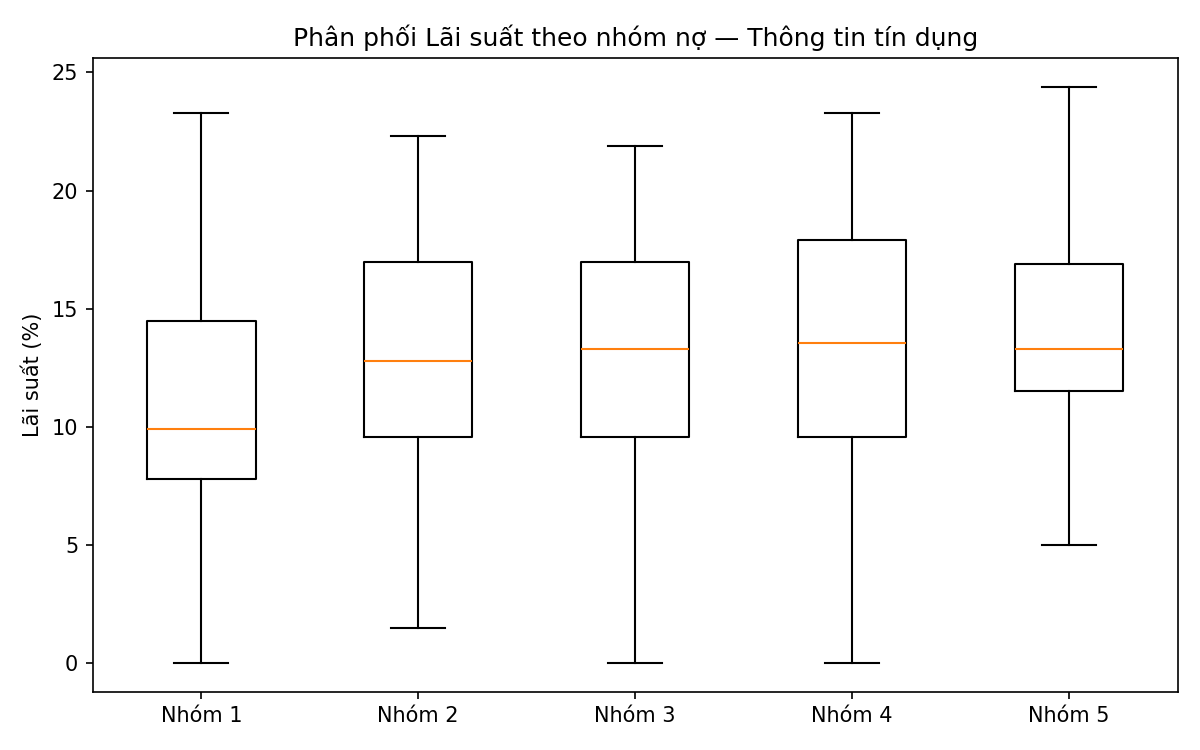
\includegraphics[width=0.7\textwidth]{figures/eda_credit_info_boxplot_laisuat.png}
\caption{Phân phối Lãi suất theo nhóm nợ — bộ dữ liệu B (kỳ 20260430)}
\label{fig:eda-b-box}
\end{figure}

Hình \ref{fig:eda-b-box} cho thấy trung vị lãi suất có xu hướng tăng từ nhóm 1 đến nhóm 5. Phân phối của nhóm 3 và nhóm 4 được ước lượng lần lượt từ 998 và 1.446 quan sát (Bảng \ref{tab:split-distribution}), qua đó hạn chế ảnh hưởng của biến động do cỡ mẫu nhỏ.

\section{Bước 3: Tiền xử lý \& chọn biến}
\label{sec:step3-preprocess}

Bước thứ ba xây dựng tập đặc trưng dùng cho huấn luyện, bao gồm loại các trường có nguy cơ rò rỉ dữ liệu, tạo đặc trưng nghiệp vụ, tính Weight of Evidence và Information Value (WOE/IV), xác lập tập đặc trưng, xử lý giá trị thiếu, mã hóa và chuẩn hóa. Mọi tham số tiền xử lý, như trung vị, trung bình, độ lệch chuẩn và danh mục mã hóa, chỉ được ước lượng trên tập huấn luyện để tránh rò rỉ thông tin từ tập kiểm định.

\subsection{Kiểm soát rò rỉ dữ liệu}
\label{sec:leakage-a}

Rò rỉ thông tin phát sinh khi biến đầu vào chứa dữ liệu chỉ xuất hiện sau thời điểm dự báo hoặc là phép biến đổi trực tiếp của biến đích. Đối với bộ A, các biến \mbox{\texttt{NHOMNO\_TCBS}} và \texttt{NHOMNO} được loại khỏi tập đầu vào; trong đó, \texttt{NHOMNO} có tương quan rất cao với \mbox{\texttt{NHOMNOMOI}}, nên việc giữ lại biến này có thể khiến mô hình tái tạo gần như trực tiếp quy tắc hình thành nhãn. Quá trình sàng lọc cũng loại biến \mbox{\texttt{DUNO\_QD}} bị trùng lặp, trường mô tả văn bản trùng với mã sản phẩm và các trường hằng số hoặc có lượng thông tin không đáng kể.

Ở bộ B, bảy trường bị loại vì có quan hệ trực tiếp với quy tắc phân loại nhóm nợ theo quy định của Ngân hàng Nhà nước: \texttt{Nhóm nợ phân loại sau khi tham chiếu CIC} (một biến thể khác của biến đích); \texttt{Dư nợ gốc chậm trả thực tế}, \texttt{Ngày chậm trả nợ gốc}, \texttt{Số tiền lãi chậm trả thực tế} và \texttt{Ngày chậm trả nợ lãi} (số ngày và số tiền chậm trả là căn cứ trực tiếp để phân loại nhóm nợ); cùng với \texttt{Dự phòng cụ thể phải trích nội bảng} và \texttt{Dự phòng cụ thể đã trích nội bảng}. Tỷ lệ trích lập dự phòng cụ thể là hàm xác định theo nhóm nợ, lần lượt bằng 0\%, 5\%, 20\%, 50\% và 100\% đối với nhóm 1 đến nhóm 5. Việc giữ các trường này có thể làm phát sinh rò rỉ thông tin, khiến mô hình tái tạo quy tắc hình thành nhãn thay vì nhận diện tín hiệu dự báo.

Đối với bài toán dự báo chuyển nhóm nợ, yêu cầu kiểm soát rò rỉ cần được thực hiện chặt chẽ hơn: mọi đặc trưng $X_{i,t}$ phải sẵn có tại hoặc trước thời điểm $t$, trong khi nhãn được xác định trong khoảng từ $t+1$ đến $t+h$. Phép chia mẫu ngẫu nhiên được sử dụng trong nghiên cứu hiện tại phù hợp với mục tiêu kiểm định mô hình phân loại trạng thái, nhưng chưa tối ưu cho bài toán cảnh báo sớm. Khi có dữ liệu theo thời gian, việc chia mẫu theo trình tự thời gian là cần thiết để ngăn thông tin tương lai tham gia quá trình huấn luyện.

\subsection{Xây dựng đặc trưng nghiệp vụ}

Hai nhánh dữ liệu sử dụng công thức tạo biến khác nhau. Bộ A tạo ba biến từ ngày mở, ngày đáo hạn, dư nợ hiện tại và dư nợ gốc. Bộ B tạo bốn biến kỹ thuật từ ngày giải ngân, ngày kết thúc khế ước và số lần cơ cấu lại thời hạn trả nợ.

Các biến này không tồn tại trực tiếp trong dữ liệu ban đầu mà được xây dựng từ một hoặc nhiều trường gốc nhằm chuyển thông tin kỹ thuật thành các đại lượng có ý nghĩa nghiệp vụ rõ ràng hơn. Bảng \ref{tab:engineered-features} tổng hợp nguồn hình thành và cách diễn giải của toàn bộ 7 biến được bổ sung.

{\footnotesize
\begin{longtable}{|p{0.6cm}|p{3.3cm}|p{3.3cm}|p{5.7cm}|}
\caption{Các biến được xây dựng thêm từ dữ liệu ban đầu}
\label{tab:engineered-features}\\
\hline
Bộ & Biến được tạo thêm & Biến gốc sử dụng & Ý nghĩa và cách diễn giải \\
\hline
\endfirsthead
\hline
Bộ & Biến được tạo thêm & Biến gốc sử dụng & Ý nghĩa và cách diễn giải \\
\hline
\endhead
A & \texttt{\seqsplit{LOAN\_TENURE\_DAYS}} & \texttt{\seqsplit{OPEN\_DATE}}, \texttt{\seqsplit{NGAYDENHAN}} & Tổng thời hạn theo hợp đồng, tính bằng số ngày từ ngày mở đến ngày đáo hạn. Giá trị lớn biểu thị khoản vay có kỳ hạn dài hơn. \\
\hline
A & \texttt{\seqsplit{DAYS\_TO\_MATURITY}} & \texttt{\seqsplit{NGAYDENHAN}}, ngày tham chiếu $d_0$ & Số ngày còn lại đến ngày đáo hạn. Giá trị dương biểu thị khoản vay chưa đáo hạn; bằng 0 là đáo hạn tại ngày tham chiếu; giá trị âm biểu thị khoản vay đã qua ngày đáo hạn. \\
\hline
A & \texttt{\seqsplit{UTIL\_RATE}} & \texttt{\seqsplit{CURR\_BAL}}, \texttt{\seqsplit{BASE\_BAL}} & Tỷ lệ giữa dư nợ hiện tại và dư nợ gốc. Giá trị gần 1 cho biết dư nợ hiện tại xấp xỉ dư nợ gốc; nhỏ hơn 1 phản ánh dư nợ đã giảm; lớn hơn 1 có thể phản ánh giải ngân bổ sung hoặc biến động số dư. \\
\hline
B & \texttt{\seqsplit{ENG\_LOAN\_AGE\_DAYS}} & \texttt{\seqsplit{ETL\_DATE}}, \texttt{Ngày giải ngân} & Số ngày đã trôi qua kể từ ngày giải ngân tới ngày chốt dữ liệu (\texttt{\seqsplit{ETL\_DATE}}) của chính hồ sơ đó, tức tuổi của khoản vay. Giá trị lớn biểu thị khoản vay đã tồn tại lâu hơn. \\
\hline
B & \texttt{\seqsplit{ENG\_DAYS\_TO\_MATURITY}} & \texttt{Ngày kết thúc khế ước}, \texttt{\seqsplit{ETL\_DATE}} & Số ngày còn lại đến ngày kết thúc khế ước, tính từ \texttt{\seqsplit{ETL\_DATE}}. Giá trị âm cho biết khế ước đã qua ngày kết thúc so với ngày chốt dữ liệu. \\
\hline
B & \texttt{\seqsplit{ENG\_TENOR\_ACTUAL\_DAYS}} & \texttt{Ngày kết thúc khế ước}, \texttt{Ngày giải ngân} & Kỳ hạn thực tế của khế ước, bằng chênh lệch giữa ngày kết thúc và ngày giải ngân. \\
\hline
B & \texttt{\seqsplit{ENG\_HAS\_RESTRUCTURE}} & \texttt{Số lần cơ cấu lại thời hạn trả nợ} & Biến nhị phân nhận giá trị 1 khi số lần cơ cấu lại thời hạn trả nợ lớn hơn 0 và nhận giá trị 0 trong trường hợp còn lại (kể cả khi thiếu dữ liệu). Biến chỉ phản ánh việc từng phát sinh cơ cấu, không cho biết mức độ. \\
\hline
\end{longtable}
}

Các biến phát sinh trên được tính hoàn toàn từ các trường đầu vào và không sử dụng biến đích. Do đó, bản thân quá trình tạo biến không trực tiếp làm lộ nhãn nhóm nợ. Tuy nhiên, trước khi triển khai thực tế, thời điểm hình thành của từng trường gốc vẫn phải được kiểm tra để bảo đảm trường đó đã tồn tại tại thời điểm dự báo; nếu một trường chỉ phát sinh sau thời điểm quan sát, biến được tạo từ trường đó vẫn có thể gây rò rỉ thông tin theo thời gian.

\subsubsection{Đặc trưng của bộ dữ liệu A}
\label{sec:feature-a}

Với ngày tham chiếu cố định $d_0=$ 31/12/2021, các biến được tính như sau:
\[
\begin{aligned}
\mathit{LOAN\_TENURE\_DAYS}_i
&=\max\{0,d_i^{\mathrm{maturity}}-d_i^{\mathrm{open}}\},\\
\mathit{DAYS\_TO\_MATURITY}_i
&=d_i^{\mathrm{maturity}}-d_0.
\end{aligned}
\]
Trong đó $d_i^{\mathrm{open}}$ là ngày mở khoản vay; $d_i^{\mathrm{maturity}}$ là ngày đến hạn; chênh lệch ngày được biểu diễn bằng số ngày dương hoặc âm. Việc cố định $d_0$ giúp cùng một hồ sơ nhận cùng giá trị khi tái chạy.

Tỷ lệ sử dụng dư nợ của bộ A được cài đặt:
\[
\mathit{UTIL\_RATE}_i
=
\begin{cases}
\operatorname{clip}\!\left(
\dfrac{\mathit{CURR\_BAL}_i}{\mathit{BASE\_BAL}_i},0,10
\right),&\mathit{BASE\_BAL}_i>0,\\
0,&\mathit{BASE\_BAL}_i\leq0.
\end{cases}
\]
Trong đó \mbox{\texttt{CURR\_BAL}} là dư nợ hiện tại; \mbox{\texttt{BASE\_BAL}} là dư nợ gốc hoặc cơ sở; và toán tử $\operatorname{clip}(x,0,10)$ giới hạn giá trị trong đoạn $[0,10]$ để giảm ảnh hưởng của tỷ số ngoại lệ.

\subsubsection{Kiểm tra đặc trưng đã tạo của bộ dữ liệu A}
\label{sec:feature-a-eda}

Sau khi ba biến \mbox{\texttt{LOAN\_TENURE\_DAYS}}, \mbox{\texttt{DAYS\_TO\_MATURITY}} và \mbox{\texttt{UTIL\_RATE}} được tạo, mục này khảo sát thống kê mô tả, ngoại lệ và tương quan của chúng cùng năm biến gốc đã trình bày ở Bước 2 (mục \ref{sec:eda}), trước khi tính Information Value ở mục sau.

\begin{table}[H]
\centering
\caption{Thống kê mô tả ba biến kỹ thuật của bộ dữ liệu A}
\label{tab:eda-a-describe-eng}
\begin{tabular}{|l|r|r|r|r|r|}
\hline
Biến & Trung bình & Độ lệch chuẩn & Nhỏ nhất & Trung vị & Lớn nhất\\
\hline
\texttt{\seqsplit{LOAN\_TENURE\_DAYS}} & 2.292,5 & 2.452,0 & 0 & 1.461 & 18.292\\
\texttt{\seqsplit{DAYS\_TO\_MATURITY}} & 672,7 & 2.397,7 & $-5.513$ & 96 & 16.798\\
\texttt{\seqsplit{UTIL\_RATE}} & 2,4561 & 3,2557 & $2\times10^{-8}$ & 0,9429 & 10,0000\\
\hline
\end{tabular}
\end{table}

\begin{table}[H]
\centering
\caption{Số quan sát ngoại lệ theo IQR — ba biến kỹ thuật của bộ dữ liệu A}
\label{tab:eda-a-outlier-eng}
\begin{tabular}{|l|r|r|}
\hline
Biến & Số ngoại lệ & Tỷ lệ (\%)\\
\hline
\texttt{\seqsplit{DAYS\_TO\_MATURITY}} & 6.233 & 23,08\\
\texttt{\seqsplit{UTIL\_RATE}} & 4.646 & 17,21\\
\texttt{\seqsplit{LOAN\_TENURE\_DAYS}} & 2.754 & 10,20\\
\hline
\end{tabular}
\end{table}

\mbox{\texttt{DAYS\_TO\_MATURITY}} có tỷ lệ ngoại lệ cao nhất (23,08\%) vì biến này nhận cả giá trị âm (khoản vay đã quá hạn đáo hạn tính đến ngày tham chiếu $d_0$) lẫn giá trị dương lớn (khoản vay kỳ hạn dài); đây là đặc điểm nghiệp vụ thực, không phải lỗi dữ liệu, nên không bị loại hay cắt ngưỡng. Ngược lại, \mbox{\texttt{UTIL\_RATE}} có 17,21\% ngoại lệ chủ yếu do một bộ phận khách hàng có dư nợ hiện tại vượt xa dư nợ gốc ban đầu (ví dụ giải ngân bổ sung nhiều lần); đây chính là lý do công thức tính \mbox{\texttt{UTIL\_RATE}} ở trên chủ động \textbf{clip} kết quả vào đoạn $[0,10]$: nếu không giới hạn, một số ít hồ sơ có tỷ lệ hàng trăm lần sẽ làm lệch cực đoan bước chuẩn hóa z-score của \emph{toàn bộ} biến này khi đưa vào Logistic Regression.

Trong nghiên cứu này, \textbf{clip dữ liệu} được hiểu là phép giới hạn giá trị của một biến trong một khoảng xác định, thay vì loại bỏ các quan sát nằm ngoài khoảng đó. Với $u$ là giá trị ban đầu của \mbox{\texttt{UTIL\_RATE}}, giá trị sau khi giới hạn được xác định như sau:
\[
\operatorname{clip}(u;0,10)=\min\{\max(u,0),10\}.
\]
Theo đó, giá trị nhỏ hơn 0 được thay bằng 0, giá trị lớn hơn 10 được thay bằng 10, còn các giá trị thuộc đoạn $[0,10]$ được giữ nguyên. Ngưỡng trên bằng 10 tương ứng với trường hợp dư nợ hiện tại bằng 10 lần dư nợ gốc. Cách xử lý này không làm giảm số lượng quan sát và vẫn bảo lưu thông tin rằng hồ sơ có mức sử dụng rất cao, đồng thời hạn chế ảnh hưởng chi phối của một số giá trị cực đoan đối với trung bình, độ lệch chuẩn và quá trình ước lượng mô hình. Tuy nhiên, sau khi giới hạn, các mức \mbox{\texttt{UTIL\_RATE}} lớn hơn 10 không còn được phân biệt với nhau; vì vậy, đây là một lựa chọn tiền xử lý nhằm tăng tính ổn định của mô hình, không hàm ý rằng các giá trị vượt ngưỡng là sai về mặt nghiệp vụ.

\begin{figure}[H]
\centering
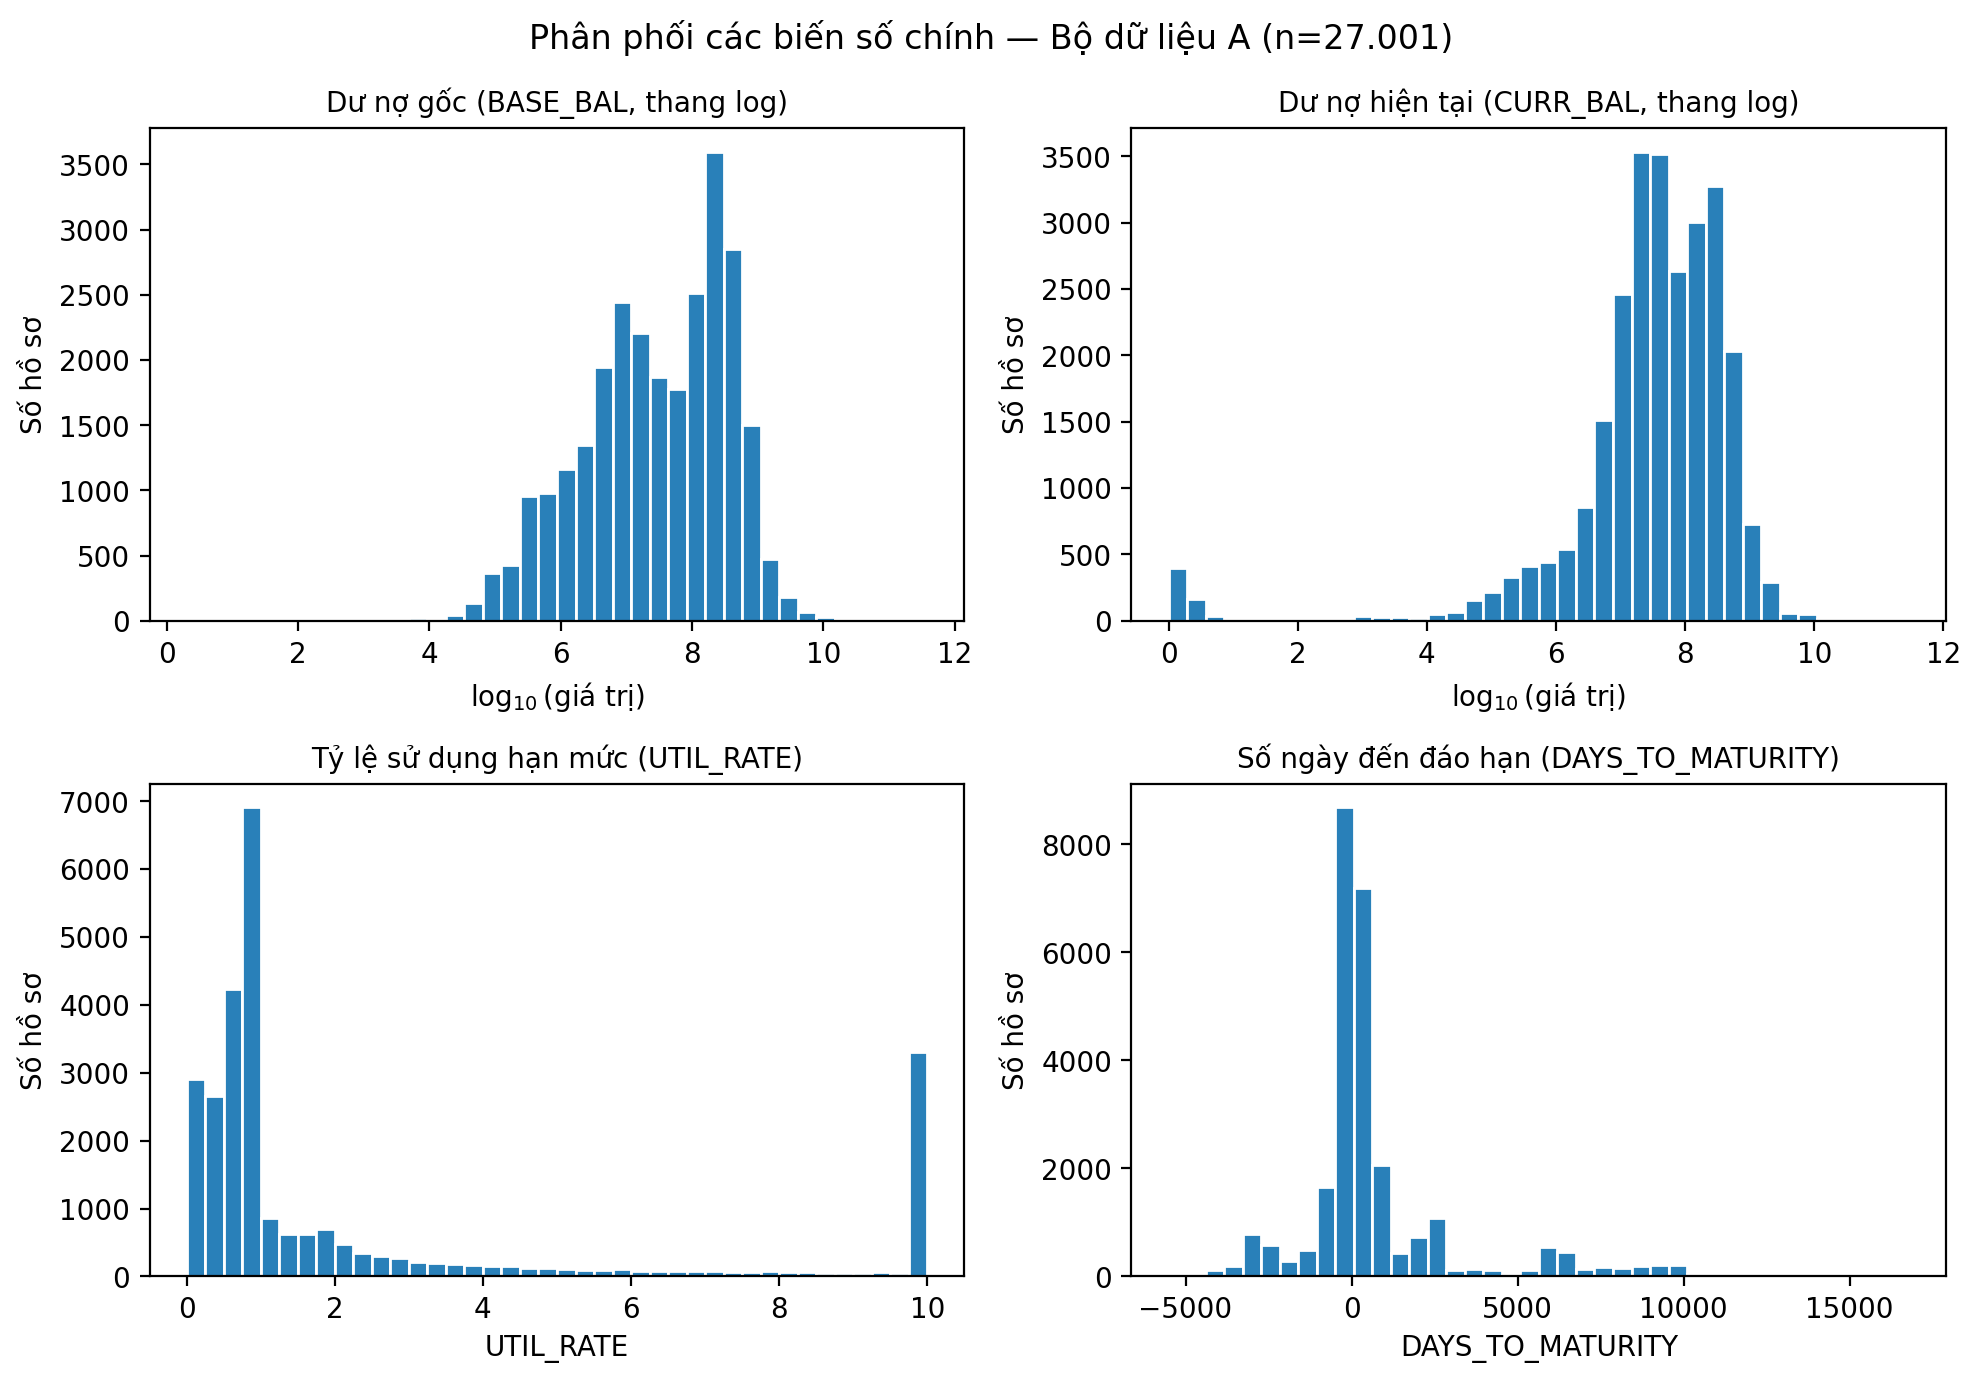
\includegraphics[width=0.95\textwidth]{figures/eda_a_histograms.png}
\caption{Phân phối bốn biến số chính của bộ dữ liệu A (n=27.001)}
\label{fig:eda-a-hist}
\end{figure}

Hình \ref{fig:eda-a-hist} minh họa trực quan hai đặc điểm đã nêu bằng số: \mbox{\texttt{BASE\_BAL}} và \mbox{\texttt{CURR\_BAL}} lệch phải mạnh trên thang gốc nên được vẽ theo $\log_{10}$ để thấy rõ hình chuông tương đối; \mbox{\texttt{UTIL\_RATE}} có một cột dồn rõ rệt tại đúng giá trị 10, bằng chứng trực quan cho thấy phép \textbf{clip} đã cắt và dồn một lượng đáng kể hồ sơ (khoảng 3.200, tương ứng phần vượt ngưỡng của 17,21\% ngoại lệ ở Bảng \ref{tab:eda-a-outlier-eng}) về đúng biên trên; \mbox{\texttt{DAYS\_TO\_MATURITY}} có hai đỉnh, một quanh 0 (khoản vay gần đáo hạn hoặc mới quá hạn) và một dải trải dài về phía dương (khoản vay kỳ hạn dài).

Ma trận tương quan (Bảng \ref{tab:eda-a-corr}, minh họa trực quan ở Hình \ref{fig:eda-a-corr}) cho thấy ba cặp biến có $|r|\geq 0,7$.

\begin{table}[H]
\centering
\caption{Các cặp biến số tương quan mạnh nhất — bộ dữ liệu A}
\label{tab:eda-a-corr}
\begin{tabular}{|l|l|r|}
\hline
Biến 1 & Biến 2 & Hệ số tương quan $r$\\
\hline
\texttt{\seqsplit{LOAN\_TENURE\_DAYS}} & \texttt{\seqsplit{DAYS\_TO\_MATURITY}} & 0,942\\
\texttt{\seqsplit{BASE\_BAL}} & \texttt{\seqsplit{CURR\_BAL}} & 0,923\\
\texttt{ORGNBR} & \texttt{\seqsplit{PARENTORGNBR}} & 0,738\\
\texttt{LAISUAT} & \texttt{\seqsplit{LOAN\_TENURE\_DAYS}} & 0,352\\
\texttt{LAISUAT} & \texttt{\seqsplit{UTIL\_RATE}} & $-0,327$\\
\hline
\end{tabular}
\end{table}

Ba cặp tương quan mạnh nhất đều có cách giải thích nghiệp vụ trực tiếp: \mbox{\texttt{LOAN\_TENURE\_DAYS}} và \mbox{\texttt{DAYS\_TO\_MATURITY}} cùng được tính từ ngày mở và ngày đáo hạn nên gần như là hai phép biến đổi tuyến tính của cùng thông tin gốc; \mbox{\texttt{CURR\_BAL}} là dư nợ hiện tại nên tương quan cao với dư nợ gốc \mbox{\texttt{BASE\_BAL}}; \texttt{ORGNBR} và \mbox{\texttt{PARENTORGNBR}} phản ánh cấu trúc phân cấp chi nhánh--đơn vị cấp trên. Mức tương quan này không đủ cao để loại biến (không có cặp nào $|r|>0,95$), nhưng đủ để giải thích vì sao trong bảng SHAP ở Chương 4, importance của hai biến kỳ hạn thường lấn át lẫn nhau tùy ngẫu nhiên hoá của mô hình cây; đây là hạn chế cố hữu khi diễn giải importance trên các biến tương quan \cite{lundberg2017unified}.

\begin{figure}[H]
\centering
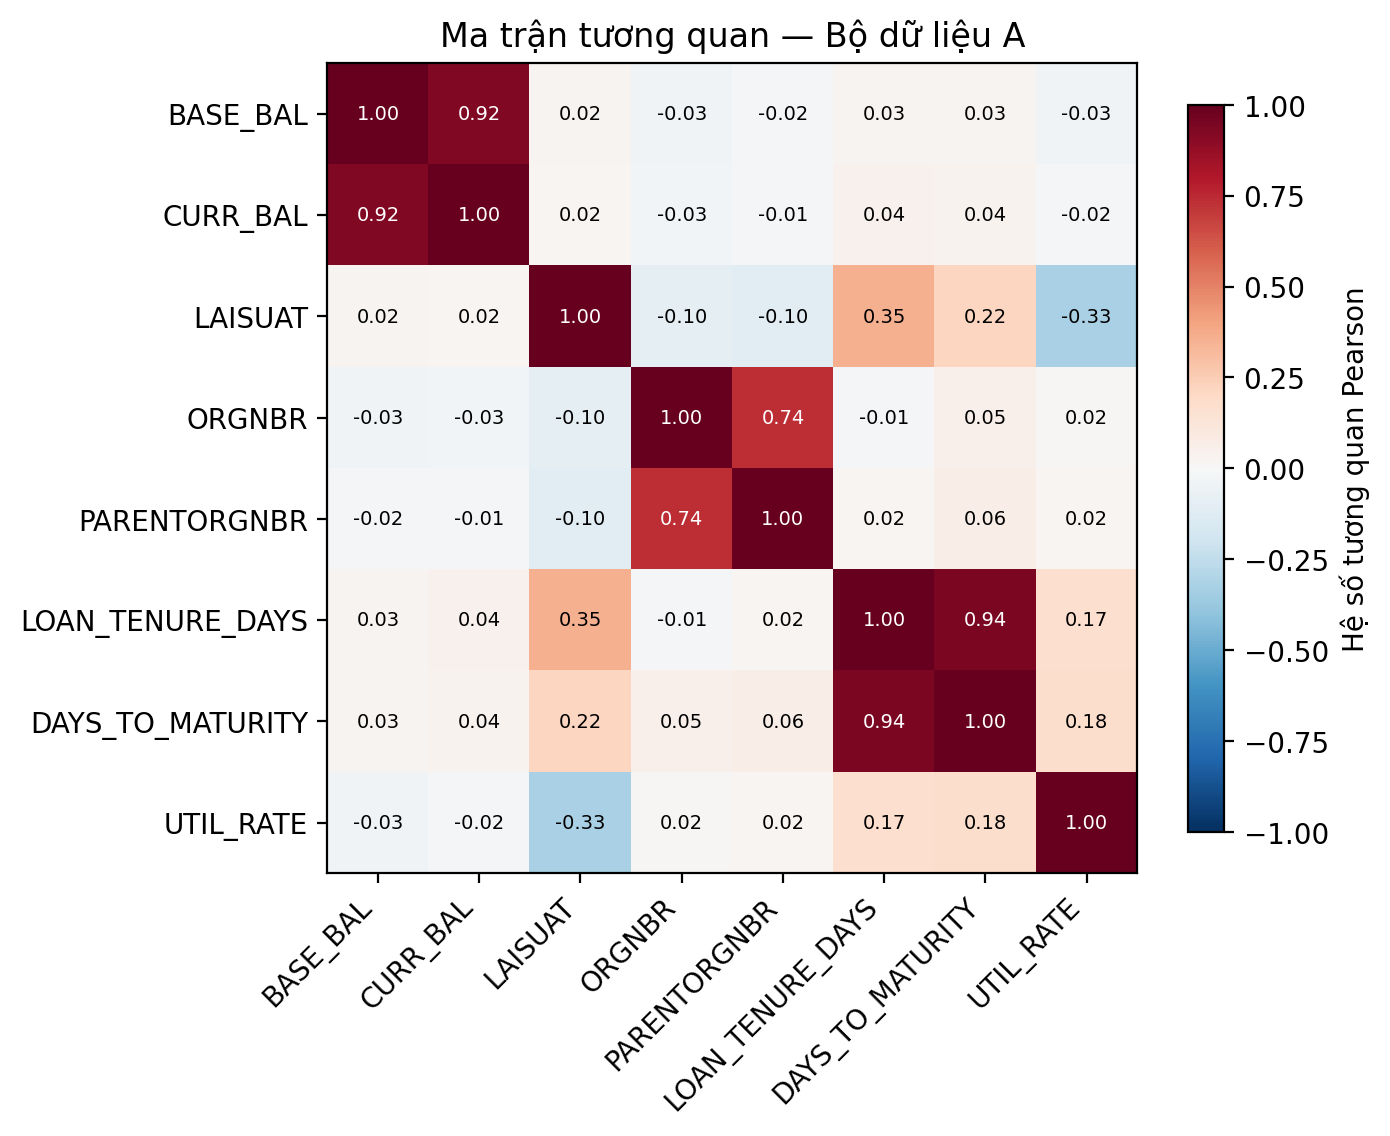
\includegraphics[width=0.75\textwidth]{figures/eda_a_correlation.png}
\caption{Ma trận tương quan Pearson giữa các biến số của bộ dữ liệu A}
\label{fig:eda-a-corr}
\end{figure}

\begin{figure}[H]
\centering
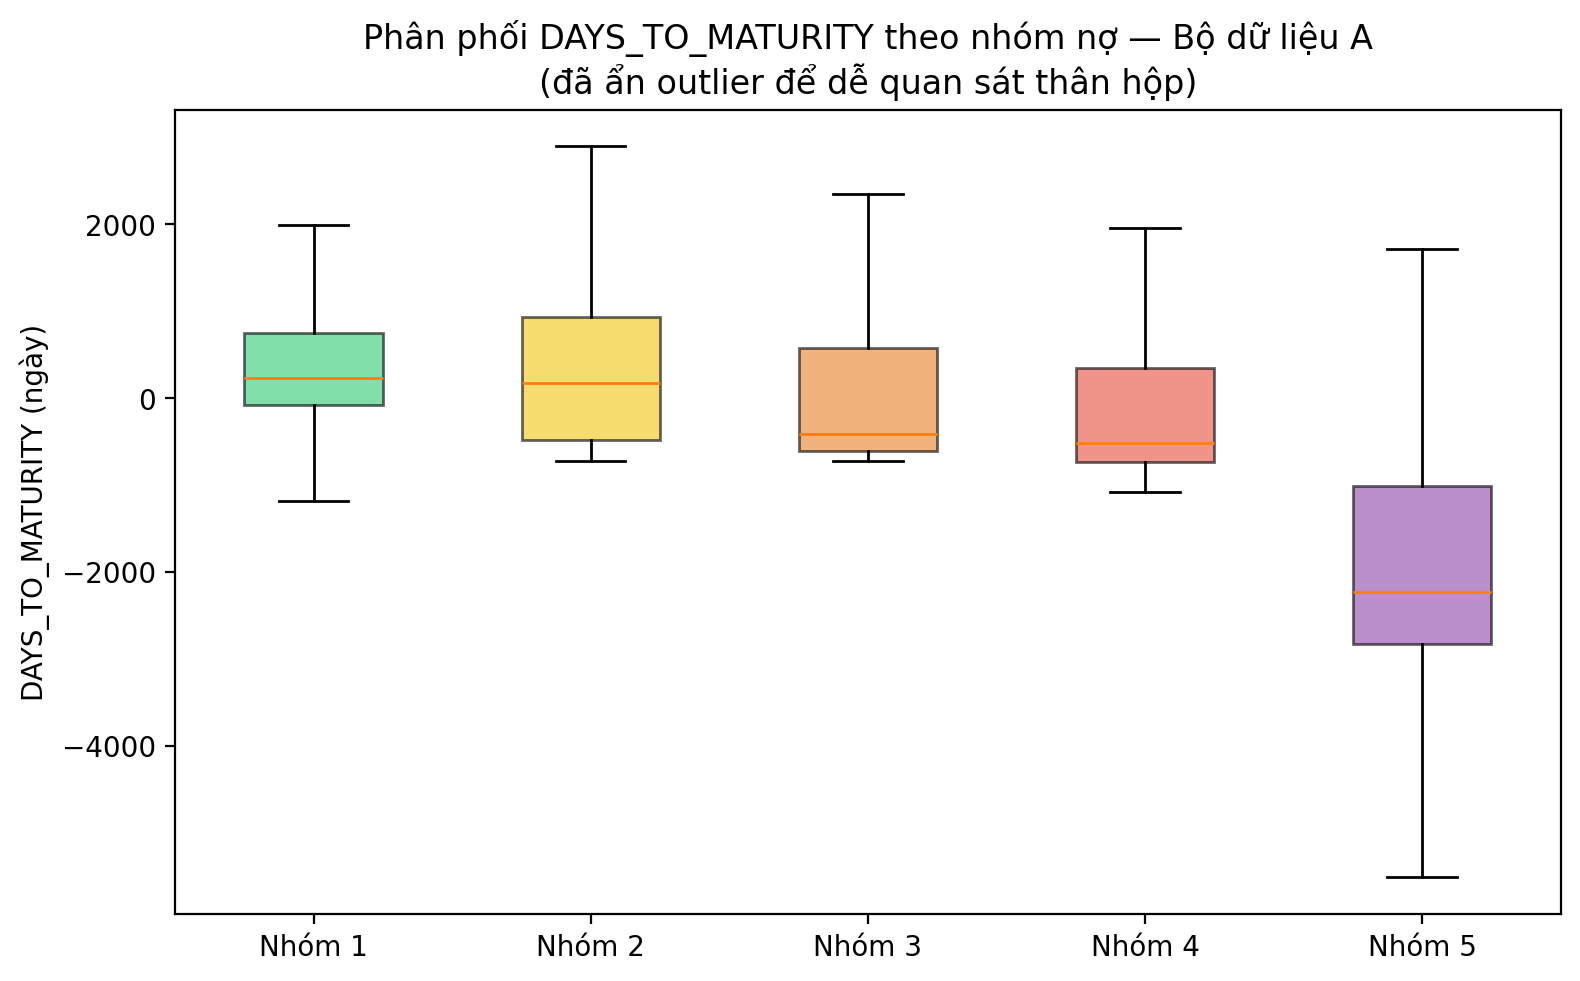
\includegraphics[width=0.7\textwidth]{figures/eda_a_boxplot_daystomaturity.png}
\caption{Phân phối \mbox{\texttt{DAYS\_TO\_MATURITY}} theo nhóm nợ — bộ dữ liệu A}
\label{fig:eda-a-box}
\end{figure}

Hình \ref{fig:eda-a-box} cho thấy trung vị \mbox{\texttt{DAYS\_TO\_MATURITY}} giảm dần khá đều từ nhóm 1 đến nhóm 4 rồi đổi hướng ở nhóm 5, phù hợp việc đây là biến SHAP xếp hạng cao nhất ở Chương 4, nhưng cũng gợi ý quan hệ giữa biến này và nhóm nợ không hoàn toàn đơn điệu, cần thận trọng khi diễn giải nhân quả.

\subsubsection{Đặc trưng thời gian của bộ dữ liệu B}
\label{sec:eng-util-b}

Ba trong bốn biến kỹ thuật của bộ B được tính bằng chênh lệch ngày, sử dụng \mbox{\texttt{ETL\_DATE}} của từng hồ sơ làm mốc tham chiếu để bảo đảm khả năng tái lập kết quả. Mỗi hồ sơ có một ngày chốt dữ liệu cố định tại thời điểm trích xuất báo cáo, nên giá trị của các biến thời gian không thay đổi khi thực thi lại mã nguồn tại một thời điểm khác. Biến còn lại được tính trực tiếp từ số lần cơ cấu lại thời hạn trả nợ.

\[
\begin{aligned}
\mathit{ENG\_LOAN\_AGE\_DAYS}_i
&= \mathit{ETL\_DATE}_i - d_i^{\mathrm{disb}},\\
\mathit{ENG\_DAYS\_TO\_MATURITY}_i
&= d_i^{\mathrm{end}} - \mathit{ETL\_DATE}_i,\\
\mathit{ENG\_TENOR\_ACTUAL\_DAYS}_i
&= d_i^{\mathrm{end}} - d_i^{\mathrm{disb}},
\end{aligned}
\]
trong đó $d_i^{\mathrm{disb}}$ là ngày giải ngân; $d_i^{\mathrm{end}}$ là ngày kết thúc khế ước; và $\mathit{ETL\_DATE}_i$ là ngày chốt dữ liệu của hồ sơ $i$. Biến nhị phân còn lại:
\[
\mathit{ENG\_HAS\_RESTRUCTURE}_i
=
\begin{cases}
1, & \mathit{SoLanCoCauLai}_i>0,\\
0, & \text{ngược lại (kể cả khi thiếu dữ liệu)}.
\end{cases}
\]

Trường \texttt{Thời điểm truy đòi}, ban đầu được xem xét làm nguồn cho một biến thời gian thứ năm, bị loại khỏi danh sách cột ngày sau khi kiểm tra thực nghiệm cho thấy trường này trùng khớp 100\% với \texttt{Ngày kết thúc khế ước} trên toàn bộ dữ liệu quan sát được; giữ lại sẽ chỉ tạo ra một biến kỹ thuật trùng lặp hoàn toàn với \mbox{\texttt{ENG\_DAYS\_TO\_MATURITY}}, không bổ sung thông tin mới.

\subsubsection{Kiểm tra đặc trưng đã tạo của bộ dữ liệu B}
\label{sec:feature-b-eda}

Cả bốn biến kỹ thuật của bộ B đều \textbf{không có giá trị thiếu} (0,00\%), vì được tính trực tiếp từ \mbox{\texttt{ETL\_DATE}}, ngày giải ngân và ngày kết thúc khế ước, ba trường có mặt ở toàn bộ 100.617 hồ sơ. Bảng \ref{tab:eda-b-describe-eng} trình bày thống kê mô tả.

\begin{table}[H]
\centering
\caption{Thống kê mô tả bốn biến kỹ thuật của bộ dữ liệu B}
\label{tab:eda-b-describe-eng}
\begin{tabular}{|l|r|r|r|r|}
\hline
Biến & Trung bình & Độ lệch chuẩn & Trung vị & Ngoại lệ IQR (\%)\\
\hline
\texttt{\seqsplit{ENG\_LOAN\_AGE\_DAYS}} & 602,82 & 632,71 & 395 & 3,05\\
\texttt{\seqsplit{ENG\_DAYS\_TO\_MATURITY}} & 1.667,40 & 2.778,31 & 711 & 11,51\\
\texttt{\seqsplit{ENG\_TENOR\_ACTUAL\_DAYS}} & 2.270,22 & 2.850,29 & 1.461 & 12,45\\
\texttt{\seqsplit{ENG\_HAS\_RESTRUCTURE}} & 0,004 & 0,063 & 0 & 0,40\\
\hline
\end{tabular}
\end{table}

\begin{figure}[H]
\centering
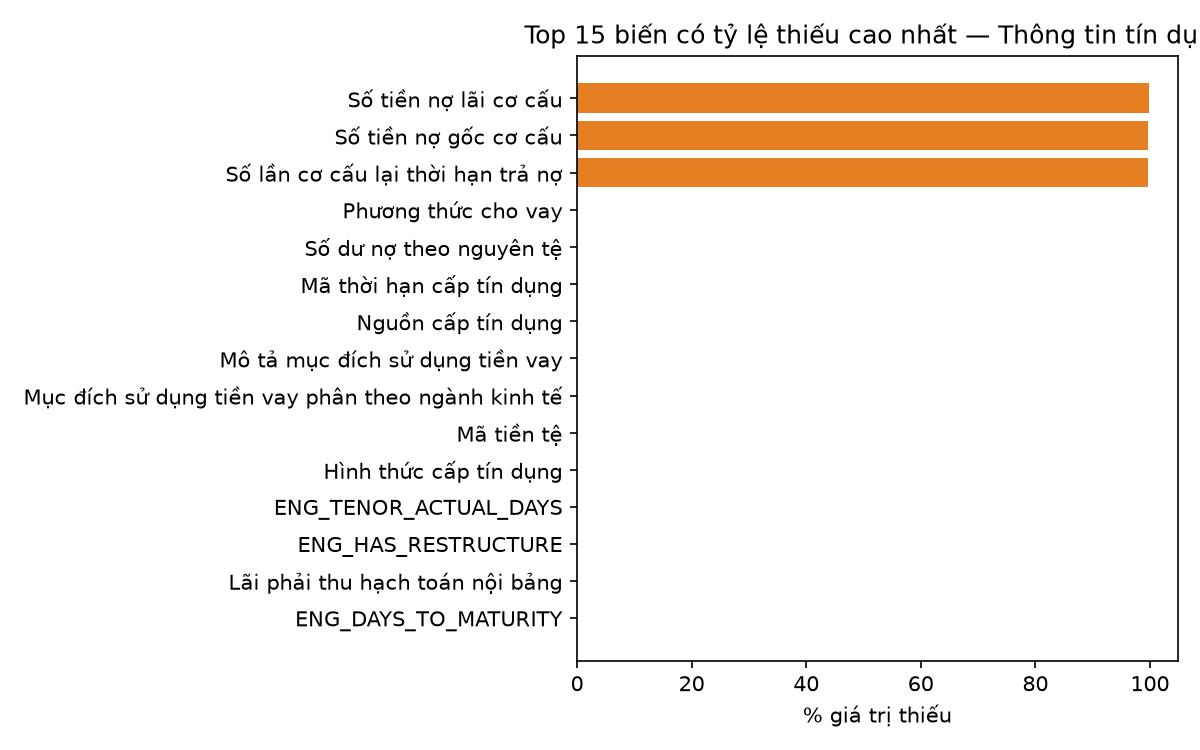
\includegraphics[width=0.85\textwidth]{figures/eda_credit_info_missing.png}
\caption{Top 15 biến (trong bể đặc trưng hợp lệ) có tỷ lệ thiếu cao nhất — bộ dữ liệu B}
\label{fig:eda-b-missing}
\end{figure}

\begin{figure}[H]
\centering
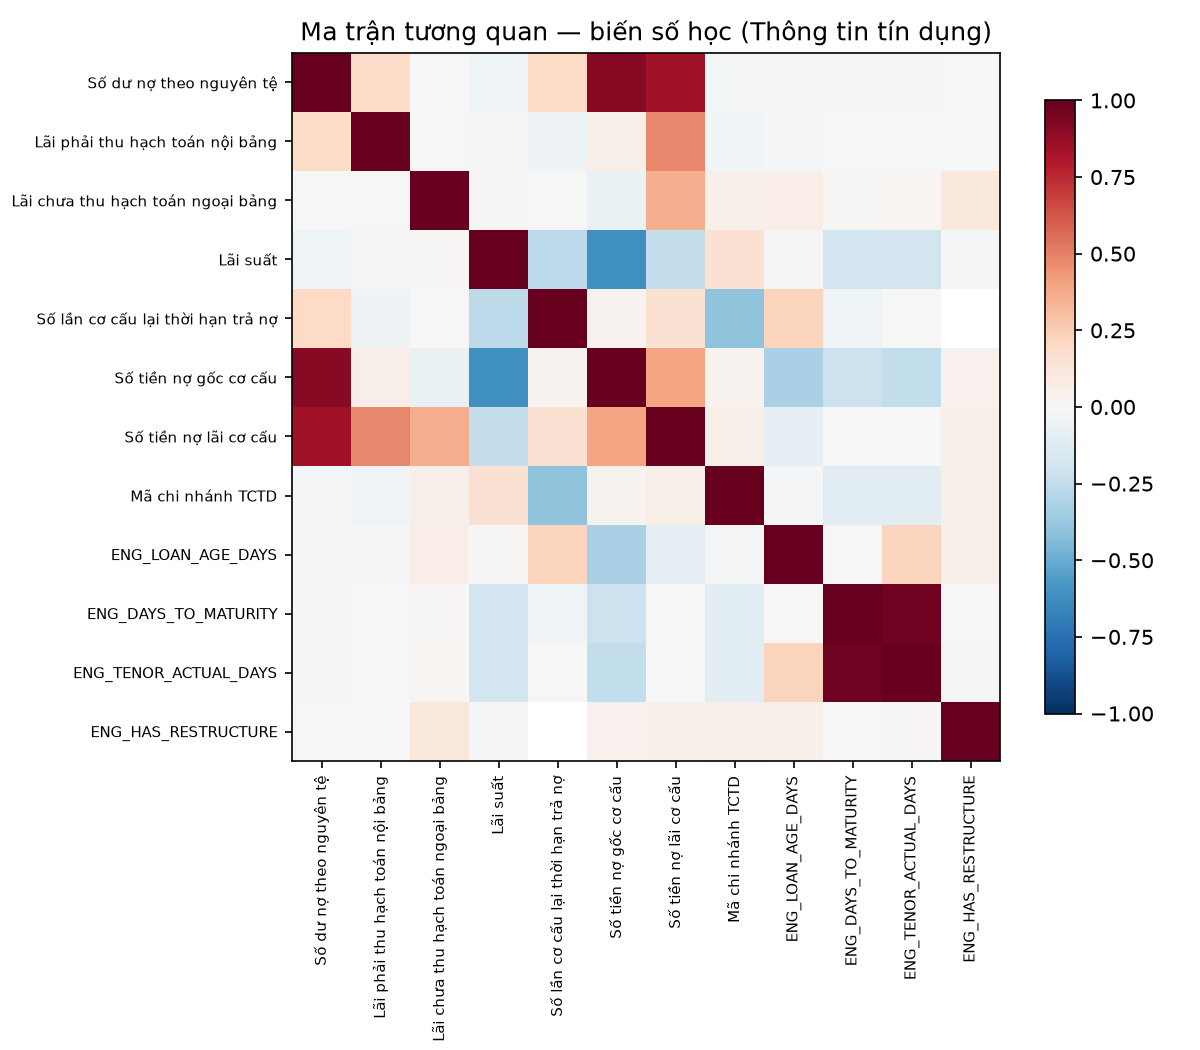
\includegraphics[width=0.8\textwidth]{figures/eda_credit_info_correlation.png}
\caption{Ma trận tương quan giữa 12 biến số (8 biến gốc + 4 biến kỹ thuật) — bộ dữ liệu B}
\label{fig:eda-b-corr}
\end{figure}

Hình \ref{fig:eda-b-corr} cho thấy cặp \mbox{\texttt{ENG\_DAYS\_TO\_MATURITY}} và \mbox{\texttt{ENG\_TENOR\_ACTUAL\_DAYS}} có hệ số tương quan lớn nhất trong 12 biến số ($r=0,975$). Mối tương quan này xuất phát từ việc cả hai đặc trưng cùng sử dụng mốc \texttt{Ngày kết thúc khế ước}, tương tự mối quan hệ giữa \mbox{\texttt{LOAN\_TENURE\_DAYS}} và \mbox{\texttt{DAYS\_TO\_MATURITY}} ở bộ A (Mục \ref{sec:feature-a-eda}). Do hệ số tương quan vượt ngưỡng tham khảo 0,95, hai biến có khả năng chứa thông tin trùng lặp đáng kể. Tuy vậy, nghiên cứu vẫn giữ lại cả hai do chúng biểu thị hai khía cạnh nghiệp vụ khác nhau, lần lượt là kỳ hạn còn lại và tổng kỳ hạn thực tế. Đây là điểm cần thận trọng khi diễn giải mức độ quan trọng ở Chương 4, bởi đóng góp của hai biến có thể cùng bắt nguồn từ một nguồn thông tin cơ sở.

\subsection{Weight of Evidence và Information Value (WOE/IV)}

Information Value (IV) được sử dụng để lượng hóa khả năng phân tách giữa nhóm nợ ``tốt'' và nhóm nợ ``xấu'' của từng biến trước khi đưa vào mô hình. Nghiên cứu quy ước nhãn nhị phân ``tốt'' tương ứng với nhóm 1 và ``xấu'' tương ứng với các nhóm 2--5; các biến số được chia thành 10 khoảng theo phân vị. IV được tính trên tập đặc trưng còn lại sau khi loại các trường có nguy cơ rò rỉ tại Mục \ref{sec:leakage-a} và bổ sung các đặc trưng nghiệp vụ, qua đó cung cấp căn cứ định lượng để xác lập tập đặc trưng tại Mục \ref{sec:pool-a}.

\subsubsection{Bảng Information Value đầy đủ của bộ dữ liệu A}
\label{sec:iv-a}

Bảng \ref{tab:iv-a} trình bày giá trị IV của toàn bộ 13 biến trong tập phân tích, bao gồm \texttt{SEX} và \texttt{LOAIKH}, theo thứ tự giảm dần. Vai trò của hai biến này trong quá trình lựa chọn tập đặc trưng được thảo luận tại Mục \ref{sec:pool-a}.

\begin{table}[H]
\centering
\caption{Information Value của 13 biến — bộ dữ liệu A}
\label{tab:iv-a}
\begin{tabular}{|l|r|l|}
\hline
Biến & IV & Mức\\
\hline
\texttt{\seqsplit{DAYS\_TO\_MATURITY}} & 4,5541 & (!) Nghi ngờ (leakage?)\\
\texttt{\seqsplit{CURRMIACCTTYPCD}} & 1,9921 & (!) Nghi ngờ (leakage?)\\
\texttt{\seqsplit{LOAN\_TENURE\_DAYS}} & 1,9410 & (!) Nghi ngờ (leakage?)\\
\texttt{\seqsplit{MUCDICHVAY}} & 1,4141 & (!) Nghi ngờ (leakage?)\\
\texttt{\seqsplit{UTIL\_RATE}} & 1,3334 & (!) Nghi ngờ (leakage?)\\
\texttt{\seqsplit{MJACCTTYPCD}} & 0,9695 & Rất mạnh\\
\texttt{LAISUAT} & 0,7851 & Rất mạnh\\
\texttt{\seqsplit{BASE\_BAL}} & 0,5356 & Rất mạnh\\
\texttt{\seqsplit{PARENTORGNBR}} & 0,3201 & Mạnh\\
\texttt{\seqsplit{CURR\_BAL}} & 0,2585 & Trung bình\\
\texttt{ORGNBR} & 0,1820 & Trung bình\\
\texttt{SEX} & 0,0081 & Vô dụng\\
\texttt{LOAIKH} & 0,0000 & Vô dụng\\
\hline
\end{tabular}
\end{table}

Kết quả cho thấy 5 trong tổng số 13 biến có $IV>1{,}0$, vượt ngưỡng mà Siddiqi xem là dấu hiệu cần thận trọng do biến có thể đại diện gián tiếp hoặc làm rò rỉ biến đích \cite{siddiqi2006credit}. Năm biến này đồng thời nằm trong nhóm có mức độ quan trọng cao nhất theo SHAP và Gain ở Chương 4. Có hai khả năng cần được phân biệt. Thứ nhất, nếu biến được tính trực tiếp từ \mbox{\texttt{NHOMNOMOI}} hoặc từ quy tắc hình thành nhãn, biến đó phải được loại tương tự \mbox{\texttt{NHOMNO}} tại Mục \ref{sec:leakage-a}. Thứ hai, nếu biến được xác lập độc lập với nhãn nhưng có quan hệ nghiệp vụ chặt chẽ với nhóm nợ, IV cao có thể phản ánh tín hiệu thực tế. Do chưa có đầy đủ thông tin về quy trình hình thành dữ liệu nguồn, kết quả này được xem là một giới hạn cần lưu ý khi diễn giải mô hình.

Luận văn nghiêng về khả năng thứ hai đối với ba biến được xây dựng trong nghiên cứu. Cụ thể, \mbox{\texttt{DAYS\_TO\_MATURITY}} phản ánh số ngày còn lại đến ngày đáo hạn; \mbox{\texttt{LOAN\_TENURE\_DAYS}} biểu thị thời hạn khoản vay; và \mbox{\texttt{UTIL\_RATE}} đo lường tỷ lệ sử dụng dư nợ. Cả ba biến đều được tính từ ngày mở khoản vay, ngày đáo hạn hoặc số dư nợ. Các trường dữ liệu nguồn này tồn tại độc lập với quy trình xếp nhóm nợ và không phải là biến phái sinh của \mbox{\texttt{NHOMNOMOI}}. Tuy nhiên, với hai biến phân loại nhiều danh mục \mbox{\texttt{CURRMIACCTTYPCD}} (31 nhóm) và \mbox{\texttt{MUCDICHVAY}} (79 nhóm), IV cao một phần có thể là hiện tượng thống kê: biến định danh có rất nhiều danh mục dễ đạt IV cao giả tạo vì mỗi danh mục nhỏ đóng góp lệch xác suất riêng, ngay cả khi không có quan hệ nhân quả mạnh; đây là hạn chế đã biết của công thức IV khi áp dụng cho biến nhiều danh mục \cite{siddiqi2006credit}. Vì vậy, luận văn khuyến nghị: (a) giữ nguyên 5 biến này trong mô hình vì không tìm thấy bằng chứng chúng được tính trực tiếp từ nhãn, nhưng (b) nêu rõ đây là hạn chế cần rà soát cùng đơn vị nghiệp vụ trước khi triển khai thực tế, đặc biệt với hai biến phân loại nhiều danh mục.

\subsubsection{Bảng Information Value của bộ dữ liệu B}
\label{sec:iv-b}

Áp dụng cùng phương pháp tính IV như bộ A (mục \ref{sec:iv-a}) cho toàn bộ 20 đặc trưng hợp lệ của bộ B. Bảng \ref{tab:iv-b-dist} tổng hợp số lượng biến theo từng mức IV; Bảng \ref{tab:iv-b-full} liệt kê chi tiết từng biến.

\begin{table}[H]
\centering
\caption{Phân bố 20 đặc trưng của bộ dữ liệu B theo mức Information Value}
\label{tab:iv-b-dist}
\begin{tabular}{|l|r|r|}
\hline
Mức IV & Số biến & Tỷ lệ (\%)\\
\hline
Vô dụng ($<0,02$) & 7 & 35,0\\
Yếu (0,02--0,1) & 6 & 30,0\\
Mạnh (0,3--0,5) & 3 & 15,0\\
Trung bình (0,1--0,3) & 2 & 10,0\\
Rất mạnh (0,5--1,0) & 1 & 5,0\\
(!) Nghi ngờ ($>1,0$) & 1 & 5,0\\
\hline
Tổng & 20 & 100,0\\
\hline
\end{tabular}
\end{table}

\begin{table}[H]
\centering
\caption{Information Value của 20 đặc trưng — bộ dữ liệu B}
\label{tab:iv-b-full}
\begin{tabular}{|l|r|l|}
\hline
Biến & IV & Mức\\
\hline
\texttt{\seqsplit{ENG\_LOAN\_AGE\_DAYS}} & 1,1170 & (!) Nghi ngờ (leakage?)\\
\texttt{Lãi phải thu hạch toán nội bảng} & 0,5420 & Rất mạnh\\
\texttt{\seqsplit{ENG\_TENOR\_ACTUAL\_DAYS}} & 0,3793 & Mạnh\\
\texttt{Mô tả mục đích sử dụng tiền vay} & 0,3611 & Mạnh\\
\texttt{Lãi suất} & 0,3130 & Mạnh\\
\texttt{\seqsplit{ENG\_DAYS\_TO\_MATURITY}} & 0,2549 & Trung bình\\
\texttt{Số dư nợ theo nguyên tệ} & 0,1892 & Trung bình\\
\texttt{Phương thức cho vay} & 0,0732 & Yếu\\
\texttt{Số tiền nợ gốc cơ cấu} & 0,0626 & Yếu\\
\texttt{Số lần cơ cấu lại thời hạn trả nợ} & 0,0620 & Yếu\\
\texttt{Mục đích sử dụng tiền vay phân theo ngành kinh tế} & 0,0620 & Yếu\\
\texttt{Mã chi nhánh TCTD} & 0,0415 & Yếu\\
\texttt{Số tiền nợ lãi cơ cấu} & 0,0320 & Yếu\\
\texttt{Mã thời hạn cấp tín dụng} & 0,0107 & Vô dụng\\
\texttt{Mã tiền tệ} & 0,0039 & Vô dụng\\
\texttt{\seqsplit{ENG\_HAS\_RESTRUCTURE}} & 0,0000 & Vô dụng\\
\texttt{Hình thức cấp tín dụng} & 0,0000 & Vô dụng\\
\texttt{Lãi chưa thu hạch toán ngoại bảng} & 0,0000 & Vô dụng\\
\texttt{Nguồn cấp tín dụng} & 0,0000 & Vô dụng\\
\texttt{Hoạt động cấp tín dụng bằng phương tiện điện tử} & 0,0000 & Vô dụng\\
\hline
\end{tabular}
\end{table}

Bảng \ref{tab:iv-b-full} cho thấy \mbox{\texttt{ENG\_LOAN\_AGE\_DAYS}}, biến kỹ thuật được xây dựng trong nghiên cứu, có IV cao nhất (1,1170), vượt ngưỡng mà Siddiqi xem là dấu hiệu cần thận trọng \cite{siddiqi2006credit}. Biến này được tính hoàn toàn từ \mbox{\texttt{ETL\_DATE}} và \texttt{Ngày giải ngân}, là hai trường tồn tại độc lập với quy tắc xếp nhóm nợ. Do đó, IV cao có thể phản ánh hiệu ứng tuổi khoản vay (\emph{seasoning effect}): khoản vay tồn tại lâu hơn có nhiều thời gian phát sinh chậm trả, trong khi khoản vay mới giải ngân thường chưa đủ thời gian để phát sinh quá hạn. Nghiên cứu giữ lại biến này nhưng không diễn giải mối liên hệ quan sát được như bằng chứng nhân quả.

Bảy trên hai mươi đặc trưng (35,0\%) có $IV<0,02$, tức ``vô dụng'' theo ngưỡng đơn biến, nhưng vẫn được giữ trong tập huấn luyện vì quy tắc lọc ở mục \ref{sec:eng-util-b} chỉ loại theo tiêu chí leakage/trùng lặp/hằng số, không lọc theo IV. Tỷ lệ này khá thấp vì bể đặc trưng đã nhỏ và tập trung (20 biến), nên ít cột dư thừa/gần hằng số.

\subsection{Xây dựng tập đặc trưng huấn luyện}
\label{sec:pool-a}

\subsubsection{Bộ dữ liệu A: tập 11 biến và tập mở rộng 13 biến}

Cấu hình huấn luyện chính sử dụng 11 đặc trưng đã qua sàng lọc, gồm ba biến phân loại và tám biến số. Để đánh giá độ nhạy của tiêu chí lựa chọn biến, tập phân tích được mở rộng lên 13 đặc trưng bằng cách bổ sung \texttt{SEX} và \texttt{LOAIKH}. Theo Bảng \ref{tab:iv-a}, hai biến này có IV lần lượt bằng 0,008 và 0,000, đều thấp hơn ngưỡng 0,02 thường được xem là không có giá trị dự báo đơn biến đáng kể \cite{siddiqi2006credit}. Việc đưa hai biến trở lại tập mở rộng nhằm kiểm tra liệu mô hình cây đa biến có thể khai thác các tương tác mà IV đơn biến không phản ánh hay không. Kết quả tại Chương 4 cho thấy sự khác biệt về hiệu quả là không đáng kể.

Sau khi phân tích ngày và tạo biến, bộ A có tám biến số:
\begin{itemize}
    \item năm biến từ tệp nguồn: \mbox{\texttt{BASE\_BAL}}, \mbox{\texttt{CURR\_BAL}}, \texttt{LAISUAT}, \texttt{ORGNBR} và \mbox{\texttt{PARENTORGNBR}};
    \item ba biến tạo thêm: \mbox{\texttt{LOAN\_TENURE\_DAYS}}, \mbox{\texttt{DAYS\_TO\_MATURITY}} và \mbox{\texttt{UTIL\_RATE}}.
\end{itemize}
Năm biến phân loại trong tập đầy đủ được chia thành:
\begin{itemize}
    \item ba biến cấu hình chính: \mbox{\texttt{MJACCTTYPCD}}, \mbox{\texttt{CURRMIACCTTYPCD}} và \mbox{\texttt{MUCDICHVAY}};
    \item hai biến IV thấp đưa lại để kiểm chứng: \texttt{SEX} và \texttt{LOAIKH}.
\end{itemize}

Đối với bộ 11 biến chính, phép đếm từ tệp nguồn là:
\[
21-1-10-2+3=11,
\]
trong đó 21 là số cột thô; 1 là biến đích; 10 là số trường trong danh sách loại; 2 là hai trường ngày chỉ dùng để tạo biến; và 3 là số biến kỹ thuật được bổ sung. Pool phân tích có 13 biến vì đưa lại hai biến \texttt{SEX} và \texttt{LOAIKH}.

\subsubsection{Bộ dữ liệu B: từ 33 cột chung tới 20 đặc trưng mô hình}

Con số 33 là số cột có mặt ở cả hai kỳ báo cáo (20260430 và 20260507), không phải số biến thực tế đưa vào bộ phân loại. Tám cột chỉ có ở kỳ 20260430 (gồm hạn mức tín dụng trên hợp đồng, trạng thái tài sản bảo đảm và các trường ngày hiệu lực/kết thúc hợp đồng) không được dùng làm đặc trưng vì tập kiểm tra độc lập 20260507 không có các cột này. Bước xây dựng bể đặc trưng từ 33 cột chung thực hiện bốn lớp lọc:

\begin{enumerate}
    \item loại biến đích;
    \item loại 4 trường định danh (mã/tên khách hàng, số hợp đồng, số khế ước) và 7 trường gây rò rỉ đã nêu ở mục \ref{sec:leakage-a} (nhóm nợ đối chiếu CIC, dư nợ/lãi chậm trả thực tế và ngày chậm trả, dự phòng cụ thể phải trích và đã trích);
    \item không đưa trực tiếp 3 trường ngày (\mbox{\texttt{ETL\_DATE}}, ngày giải ngân, ngày kết thúc khế ước) vào mô hình; các trường này chỉ dùng để tạo 4 biến thời gian ở mục \ref{sec:eng-util-b}. Loại thêm 1 trường ngày trùng lặp hoàn toàn (\texttt{Thời điểm truy đòi}) và 1 cột hằng số (\texttt{Số tiền đã thanh toán}, toàn bộ giá trị bằng 0 trong dữ liệu quan sát được).
\end{enumerate}

Sau quá trình sàng lọc, tập dữ liệu còn 8 biến số và 8 biến phân loại. Bước xây dựng đặc trưng nghiệp vụ bổ sung 4 biến số, đưa tổng số biến đầu vào lên:
\[
p=8+8+4=20.
\]
Tương đương, phép đếm từ tệp nguồn có thể viết:
\[
33-1-4-7-4-1+4=20.
\]
Trong đó, 1 là biến đích; 4 là số trường định danh; 7 là số trường có nguy cơ rò rỉ thông tin; 4 là số trường ngày (3 dùng để sinh đặc trưng, 1 trùng lặp bị loại); 1 là cột hằng số; và 4 là số biến được xây dựng thêm. Ràng buộc 33 cột chung giữa hai kỳ báo cáo đã tự nhiên giới hạn bể đặc trưng ở quy mô nhỏ và tập trung (20 đặc trưng), khiến câu hỏi ``có thể giảm còn bao nhiêu đặc trưng'' ở Chương 4 mang ý nghĩa thực tiễn trực tiếp hơn: bể đặc trưng ban đầu vốn đã không có nhiều dư thừa cần cắt bớt.

\begin{figure}[H]
\centering
\begin{tabular}{c@{\hspace{4mm}$\longrightarrow$\hspace{4mm}}c@{\hspace{4mm}$\longrightarrow$\hspace{4mm}}c}
\fbox{\parbox[c][1.5cm][c]{3.4cm}{\centering 41 cột dữ liệu huấn luyện\\33 cột chung giữa hai kỳ}} &
\fbox{\parbox[c][1.5cm][c]{4.0cm}{\centering 20 đặc trưng hợp lệ\\8 số + 8 phân loại + 4 tạo thêm}} &
\fbox{\parbox[c][1.5cm][c]{4.1cm}{\centering Cấu hình rút gọn\\8 biến quan trọng nhất (Chương 4)}}
\end{tabular}
\caption{Các tầng số lượng biến trong nghiên cứu}
\label{fig:feature-reduction-levels}
\end{figure}

Đối với bộ B, nghiên cứu không xác lập trước một tập đặc trưng rút gọn cố định. Toàn bộ 20 đặc trưng hợp lệ được sử dụng trong cấu hình huấn luyện chính; khả năng rút gọn được đánh giá thông qua thực nghiệm sử dụng $k$ đặc trưng có mức độ quan trọng cao nhất, trình bày tại Chương 4.

\subsubsection{Nhóm đặc trưng nghiệp vụ}

Đối với bộ A, 13 biến được phân vào sáu nhóm: Dư nợ và hạn mức sử dụng; Lãi suất; Kỳ hạn khoản vay; Đơn vị/chi nhánh; Sản phẩm và mục đích vay; Nhân khẩu học có IV thấp. Đối với bộ B, 20 biến được phân vào sáu nhóm: (1) Dư nợ \& Thanh toán; (2) Lãi suất; (3) Kỳ hạn \& Cơ cấu lại; (4) Hình thức \& Mục đích vay; (5) Chi nhánh; và (6) Đặc trưng kỹ thuật.

Việc phân nhóm biến phục vụ hai mục đích: giải thích mô hình ở cấp độ nghiệp vụ và xây dựng khuyến nghị đầu tư dữ liệu. Tuy nhiên, tổng mức độ quan trọng của một nhóm chỉ phản ánh cách mô hình sử dụng dữ liệu hiện có và không cung cấp bằng chứng về quan hệ nhân quả.

\subsection{Giá trị thiếu và chuẩn hóa}

Đối với biến số, \mbox{\texttt{SimpleImputer(strategy="median")}} thay giá trị thiếu bằng trung vị học trên tập huấn luyện:
\[
\tilde{x}_{ij}=
\begin{cases}
x_{ij},&x_{ij}\ \text{quan sát được},\\
\operatorname{median}\{x_{\ell j}:\ell\in\mathcal{T}\},&x_{ij}\ \text{thiếu},
\end{cases}
\]
trong đó $x_{ij}$ là giá trị biến $j$ của quan sát $i$; $\mathcal{T}$ là tập chỉ số huấn luyện; và $\tilde{x}_{ij}$ là giá trị sau điền khuyết.

Đối với Logistic Regression, Decision Tree, Random Forest, XGBoost và LightGBM, biến số sau điền khuyết được chuẩn hóa:
\[
z_{ij}=\frac{\tilde{x}_{ij}-\mu_j}{\sigma_j},
\]
trong đó $\mu_j$ và $\sigma_j$ lần lượt là trung bình và độ lệch chuẩn của biến $j$ sau điền khuyết trên tập huấn luyện; $z_{ij}$ là giá trị chuẩn hóa. Việc chuẩn hóa đặc biệt cần cho hồi quy logistic, còn mô hình cây ít nhạy hơn với thang đo \cite{bishop2006pattern,hosmer2013applied}.

\subsection{Biến phân loại}

Đối với Logistic Regression, Decision Tree, Random Forest, XGBoost và LightGBM, mã nguồn sử dụng một bộ \mbox{\texttt{LabelEncoder}} riêng cho từng cột. Nếu xuất hiện giá trị mới chưa có trong tập huấn luyện, giá trị đó được ánh xạ về lớp đầu tiên của bộ mã hóa. Cách xử lý này bảo đảm khả năng thực thi nhưng có thể tạo ra thứ tự không có ý nghĩa đối với biến định danh; đây là một hạn chế của quy trình tiền xử lý cần được lưu ý khi diễn giải kết quả.

CatBoost sử dụng preprocessor riêng: biến số chỉ được điền trung vị, không chuẩn hóa; biến phân loại thiếu được thay bằng \texttt{UNKNOWN} và giữ dạng chuỗi để thuật toán xử lý trực tiếp, phù hợp cơ chế của CatBoost \cite{prokhorenkova2018catboost}.

Việc sử dụng trung vị thay cho trung bình ở bước điền khuyết được lựa chọn dựa trên kết quả phân tích khám phá tại mục \ref{sec:eda}. Các biến tiền tệ trong cả hai bộ dữ liệu có phân phối lệch phải mạnh (Bảng \ref{tab:eda-a-describe}, \ref{tab:eda-b-describe}), độ lệch chuẩn lớn hơn giá trị trung bình nhiều lần và tỷ lệ ngoại lệ theo IQR đáng kể. Trung vị ít nhạy cảm hơn với ngoại lệ và phân phối lệch, trong khi trung bình có thể bị chi phối bởi các giá trị cực lớn, khiến giá trị điền khuyết kém đại diện cho phần lớn hồ sơ \cite{bishop2006pattern}.

\subsection{Ví dụ minh họa trước và sau xử lý}
\label{sec:preprocessing-examples}

Để minh họa các phép biến đổi nêu trên, Bảng \ref{tab:example-a} trình bày ba hồ sơ thực tế trong tập kiểm định của bộ A qua từng bước xử lý.

\begin{table}[H]
\centering
\caption{Ví dụ ba hồ sơ thực tế của bộ A trước và sau xử lý}
\label{tab:example-a}
\begin{tabular}{|l|r|r|r|}
\hline
Biến & Hồ sơ \#5944 & Hồ sơ \#7333 & Hồ sơ \#12595\\
\hline
\multicolumn{4}{|l|}{\textit{Giá trị thô (không có biến nào thiếu ở bộ A)}}\\
\hline
\texttt{\seqsplit{BASE\_BAL}} & 201.000.000 & 5.000.000 & 300.000.000\\
\texttt{\seqsplit{CURR\_BAL}} & 77.050.000 & 9.184.112 & 180.000.000\\
\texttt{LAISUAT} & 0,1173 & 0,0000 & 0,1200\\
\texttt{\seqsplit{UTIL\_RATE}} & 0,3833 & 1,8368 & 0,6000\\
\texttt{\seqsplit{MJACCTTYPCD}} & CNS & CNS & CNS\\
\texttt{\seqsplit{CURRMIACCTTYPCD}} & TH01 & VS01 & TH01\\
\hline
\multicolumn{4}{|l|}{\textit{Sau chuẩn hóa z-score (học $\mu,\sigma$ trên tập huấn luyện)}}\\
\hline
\texttt{\seqsplit{BASE\_BAL}} & $-0,0334$ & $-0,0651$ & $-0,0173$\\
\texttt{\seqsplit{CURR\_BAL}} & $-0,0501$ & $-0,0628$ & $-0,0310$\\
\texttt{LAISUAT} & 0,7095 & $-1,0111$ & 0,7491\\
\texttt{\seqsplit{UTIL\_RATE}} & $-0,6374$ & $-0,1923$ & $-0,5710$\\
\hline
\multicolumn{4}{|l|}{\textit{Sau mã hóa LabelEncoder (học trên tập huấn luyện)}}\\
\hline
\texttt{\seqsplit{MJACCTTYPCD}} & 1 & 1 & 1\\
\texttt{\seqsplit{CURRMIACCTTYPCD}} & 12 & 22 & 12\\
\hline
\end{tabular}
\end{table}

Vì bộ A không có giá trị thiếu, bước điền khuyết không làm thay đổi số liệu; bảng chỉ còn ý nghĩa với các bộ dữ liệu khác có \textit{NaN}. Điểm đáng chú ý là hồ sơ \#7333 có \mbox{\texttt{UTIL\_RATE}} thô bằng 1,8368 (dư nợ hiện tại đã vượt 183,7\% dư nợ gốc), sau chuẩn hóa cho z-score $-0,1923$, âm dù bản thân tỷ lệ sử dụng cao hơn hai hồ sơ còn lại, vì \mbox{\texttt{UTIL\_RATE}} trung bình toàn mẫu huấn luyện xấp xỉ 2,46 (Bảng \ref{tab:eda-a-describe-eng}); đây là lý do luận văn nhấn mạnh z-score chỉ có ý nghĩa \emph{tương đối} trong phân phối đã lệch, không nên diễn giải như một chỉ số rủi ro tuyệt đối.

Bảng \ref{tab:example-b} minh họa ba hồ sơ thực tế của bộ B có giá trị thiếu tại biến \texttt{Phương thức cho vay}. Trong dữ liệu gốc, biến này thiếu ở 46 trong tổng số 100.617 hồ sơ, tương ứng 0,05\%.

\begin{table}[H]
\centering
\caption{Ví dụ ba hồ sơ thực tế của bộ B có giá trị thiếu, trước và sau xử lý}
\label{tab:example-b}
\begin{tabular}{|l|r|r|r|}
\hline
Biến & Hồ sơ \#22771 & Hồ sơ \#26934 & Hồ sơ \#26961\\
\hline
\multicolumn{4}{|l|}{\textit{Giá trị thô}}\\
\hline
\texttt{Số dư nợ theo nguyên tệ} & 338 & 13.700 & 8.840\\
\texttt{Lãi suất} & 16,50 & 16,95 & 21,00\\
\texttt{Phương thức cho vay} & \textit{NaN} & \textit{NaN} & \textit{NaN}\\
\texttt{Nhóm nợ tự phân loại} & 5 & 5 & 5\\
\hline
\multicolumn{4}{|l|}{\textit{Sau chuẩn hóa z-score (học $\mu,\sigma$ trên tập huấn luyện)}}\\
\hline
\texttt{Số dư nợ theo nguyên tệ} & $-0,0390$ & 0,0706 & 0,0307\\
\texttt{Lãi suất} & 1,2578 & 1,3667 & 2,3438\\
\hline
\multicolumn{4}{|l|}{\textit{Sau điền khuyết (most\_frequent) / mã hóa}}\\
\hline
\texttt{Phương thức cho vay} & 11 & 11 & 11\\
\hline
\end{tabular}
\end{table}

Cả ba hồ sơ trong ví dụ đều thuộc nhóm nợ 5 và có \texttt{Phương thức cho vay} thiếu; cỡ mẫu nhỏ nên chưa đủ để khẳng định giá trị thiếu ở biến này tương quan với nhóm nợ, nhưng là điểm cần theo dõi thêm khi có nhiều dữ liệu hơn. Với \mbox{\texttt{SimpleImputer(strategy="most\_frequent")}}, giá trị thiếu được thay bằng danh mục xuất hiện nhiều nhất trên tập huấn luyện, mã \texttt{11} (chiếm 76,9\% trong ba giá trị hợp lệ \texttt{11}/\texttt{14}/\texttt{16} của biến này), trước khi đưa qua \mbox{\texttt{LabelEncoder}} như các mô hình còn lại; với CatBoost, giá trị thiếu được giữ dạng chuỗi \texttt{UNKNOWN} thay vì điền most\_frequent, theo đúng preprocessor riêng đã mô tả ở mục sau. Ba biến số trong bảng cũng cho thấy cùng hiệu ứng nén biến thiên sau chuẩn hóa đã nêu ở ví dụ bộ A: dù \texttt{Số dư nợ theo nguyên tệ} của hồ sơ \#26934 (13.700) lớn gấp hơn 40 lần hồ sơ \#22771 (338), z-score tương ứng chỉ chênh lệch khoảng 0,11, do độ lệch chuẩn toàn mẫu (121.908,73) lớn hơn nhiều so với trung bình (5.092,31).

\subsection{Phân tích số lượng và nhóm đặc trưng}

Trong cấu hình phân tích, XGBoost được sử dụng để xác lập thứ hạng mức độ quan trọng của đặc trưng riêng cho từng bộ dữ liệu. Với các đặc trưng được sắp xếp sao cho $I_{(1)}\geq\cdots\geq I_{(p)}$, tỷ lệ mức độ quan trọng tích lũy tại $k$ được xác định như sau:
\[
Q(k)=\frac{\sum_{j=1}^{k}I_{(j)}}{\sum_{j=1}^{p}I_{(j)}}\times100\%.
\]
Trong đó $I_{(j)}$ là mức độ quan trọng của đặc trưng có thứ hạng $j$; $p=13$ đối với tập đầy đủ của bộ A và $p=20$ đối với bộ B. Đại lượng $Q(k)$ phản ánh tỷ lệ mức độ quan trọng tích lũy, không phải tỷ lệ hiệu quả dự báo được duy trì. Vì vậy, số biến đạt 95\% mức độ quan trọng chỉ được xem là cấu hình ứng viên và phải được huấn luyện, đánh giá lại trên dữ liệu ngoài mẫu. Các giá trị khảo sát là $k\in\{3,5,7,9,11,13\}$ đối với bộ A và $k\in\{3,5,8,11,14,17,20\}$ đối với bộ B.

Đóng góp của nhóm đặc trưng $g$ được xác định theo công thức:
\[
I_g=\sum_{j:\,g(j)=g}I_j,\qquad
S_g=\frac{I_g}{\sum_{r}I_r}\times100\%,
\]
trong đó $g(j)$ ánh xạ đặc trưng $j$ vào nhóm nghiệp vụ tương ứng; $I_g$ là tổng mức độ quan trọng và $S_g$ là tỷ trọng của nhóm.

Chỉ số ưu tiên dữ liệu được xác định như sau:
\label{sec:priority-formula}
\[
\mathrm{Priority}_g=S_g\left(\frac{M_g}{100}+0,1\right),
\]
trong đó $M_g$ là tỷ lệ thiếu trung bình của nhóm $g$ và 0,1 là hệ số nền do tác giả quy ước. Chỉ số này chỉ có vai trò hỗ trợ sắp xếp nội dung thảo luận, chưa phải là một hàm lợi ích kinh tế đã được hiệu chỉnh và kiểm định.

Phương pháp lựa chọn biến có hai giới hạn cần lưu ý. Thứ nhất, nhiều giá trị $k$ được khảo sát trên cùng một tập kiểm định trước khi lựa chọn cấu hình có kết quả cao nhất, do đó có thể phát sinh thiên lệch lựa chọn. Các đường cong hiệu quả theo $k$ chỉ được sử dụng cho mục đích phân tích khám phá, không được xem là kết quả của một quy trình lựa chọn biến đã kiểm định độc lập. Thứ hai, tổng mức độ quan trọng theo nhóm không thể thay thế thực nghiệm loại bỏ lần lượt từng nhóm đặc trưng.

\section{Bước 4: Chia dữ liệu \& cân bằng lớp}
\label{sec:step4-split-balance}

Bước thứ tư chia dữ liệu thành tập huấn luyện và kiểm định theo nguyên tắc phân tầng, sau đó xử lý mất cân bằng lớp chỉ trên tập huấn luyện.

\subsection{Chia tập huấn luyện--kiểm định}

Mã nguồn đặt tham số \mbox{\texttt{RANDOM\_STATE=42}}, tỷ lệ kiểm định bằng 0,2 và thực hiện phép chia ngẫu nhiên có phân tầng theo nhãn. Bộ dữ liệu A được chia thành 21.600 quan sát huấn luyện và 5.401 quan sát kiểm định. Bộ dữ liệu B (kỳ 20260430) được chia thành 80.493 quan sát huấn luyện và 20.124 quan sát kiểm định (Bảng \ref{tab:split-distribution}); ngoài ra, toàn bộ 100.274 quan sát của kỳ 20260507 được giữ lại làm tập kiểm tra độc lập, không tham gia bước chia phân tầng này (mục \ref{sec:dataset-b-structure}).

Mô hình phân loại nhóm nợ được đánh giá theo hai tầng. Tầng thứ nhất sử dụng phép chia huấn luyện--kiểm định theo tỷ lệ 80/20 để so sánh các mô hình trong cùng điều kiện. Tầng thứ hai sử dụng kiểm định chéo phân tầng lặp lại (\textit{Repeated Stratified K-Fold}), được trình bày chi tiết tại Mục \ref{sec:repeated-cv}. Với $R=3$ lần lặp và $F=5$ phần, mô hình được ước lượng $R\times F=15$ lần; mỗi quan sát xuất hiện trong phần kiểm định đúng một lần ở mỗi lượt lặp. Thiết kế này không làm tăng số quan sát thực tế, nhưng giúp giảm mức độ phụ thuộc của Recall ở các lớp hiếm vào một lần chia mẫu duy nhất.

\subsection{Xử lý mất cân bằng lớp}
\label{sec:imbalance}

SMOTE tạo một điểm tổng hợp:
\[
\mathbf{x}_{\mathrm{new}}
=
\mathbf{x}_i+\lambda\left(\mathbf{x}_{nn}-\mathbf{x}_i\right),
\qquad \lambda\sim U(0,1),
\]
trong đó $\mathbf{x}_i$ là véc-tơ của một quan sát lớp thiểu số; $\mathbf{x}_{nn}$ là một trong các láng giềng gần của nó; $\lambda$ là số ngẫu nhiên phân bố đều trên $[0,1]$; và $\mathbf{x}_{\mathrm{new}}$ là điểm nội suy \cite{chawla2002smote}.

Đối với bộ A, chiến lược \mbox{\texttt{smote\_moderate}} nâng số quan sát huấn luyện của các lớp 2, 3, 4 và 5 từ 1.030, 483, 627 và 2.689 lên lần lượt 3.000, 2.000, 2.000 và 5.000. Đối với bộ B, chiến lược tùy chỉnh nâng số quan sát của bốn lớp tương ứng từ 5.057, 798, 1.157 và 2.382 lên 8.000, 4.000, 4.500 và 6.000. Sau lấy mẫu, quy mô các lớp thiểu số tương đương khoảng 5,6--11,2\% lớp đa số, trong khi tỷ trọng quan sát tổng hợp trong từng lớp vẫn dưới 50\%. SMOTE được thực hiện sau bước tiền xử lý và trước bước huấn luyện mô hình, đồng thời chỉ tác động đến tập huấn luyện.

\subsubsection{Ví dụ minh họa SMOTE trên nhóm 3 của bộ B}

Nhóm 3 (nợ dưới tiêu chuẩn) của bộ B có 798 hồ sơ thực tế trong tập huấn luyện. Xét hai hồ sơ thuộc nhóm này, trong đó hồ sơ thứ nhất là $\mathbf{x}_i$ (\texttt{Lãi suất}=6,85) và hồ sơ lân cận là $\mathbf{x}_{nn}$ (\texttt{Lãi suất}=12,39). Với $\lambda=0,5$, công thức SMOTE cho kết quả:
\[
x_{\mathrm{new}}
= 6,85 + 0,5\times(12,39-6,85)
= 9,62.
\]
Quan sát tổng hợp không tồn tại trong dữ liệu gốc mà nằm trên đoạn thẳng nối hai hồ sơ cùng nhóm 3 trong không gian đặc trưng đã chuẩn hóa. Đây là cơ chế được SMOTE sử dụng để tăng số quan sát huấn luyện của nhóm 3 từ 798 lên 4.000 theo chiến lược tùy chỉnh. Do nhóm 3 có số lượng quan sát gốc tương đối lớn và thể hiện biến thiên trên phần lớn các đặc trưng, nguy cơ các quan sát tổng hợp không tạo thêm biến thiên có ý nghĩa được đánh giá là không đáng kể trong bộ dữ liệu này.

Code mới còn cho phép học theo chi phí bằng trọng số lớp:
\[
w_c=\frac{N}{K\,n_c},
\]
trong đó $N$ là số quan sát huấn luyện, $K$ là số lớp và $n_c$ là số quan sát thuộc lớp $c$. Mỗi quan sát $i$ được gán trọng số $w_{y_i}$. Đối với XGBoost, trọng số được tính lại trong từng phần huấn luyện của kiểm định chéo thông qua \mbox{\texttt{compute\_sample\_weights()}}, nhờ đó không sử dụng tần suất lớp của phần kiểm định. Đối với CatBoost, các chiến lược cân bằng khác \texttt{none} được ánh xạ sang cơ chế \mbox{\texttt{auto\_class\_weights=Balanced}}; SMOTE không được áp dụng trực tiếp trên các biến phân loại dạng chuỗi.

Hai lưu ý cần nêu rõ. Thứ nhất, biến phân loại đã label-encode được SMOTE nội suy như biến số, có thể sinh giá trị không tương ứng danh mục thực. Thứ hai, trang phân tích Top-$k$ của bộ B gọi chiến lược \mbox{\texttt{smote\_moderate}}, khác với chiến lược tùy chỉnh của bảng mô hình đầy đủ. Do đó, so sánh số tuyệt đối giữa hai bảng còn chịu ảnh hưởng của chiến lược lấy mẫu. Tài liệu cho thấy xử lý mất cân bằng có thể làm thay đổi thứ hạng mô hình và không có một kỹ thuật luôn tốt nhất \cite{brown2012experimental}.

\section{Bước 5: Huấn luyện mô hình}
\label{sec:step5-train}

Bước thứ năm huấn luyện và tinh chỉnh các mô hình phân loại, đồng thời mô tả cách mô hình được lưu trữ, triển khai phục vụ ứng dụng, và định hướng giám sát vận hành sau này.

\subsection{Xây dựng mô hình}
\label{sec:models}

Mã nguồn cài đặt Logistic Regression, Decision Tree, Random Forest, XGBoost, LightGBM và CatBoost. Các tham số chính gồm:

\begin{itemize}
    \item Decision Tree: độ sâu tối đa 10, tối thiểu 10 mẫu ở lá;
    \item Random Forest: 300 cây, độ sâu tối đa 15, tối thiểu 5 mẫu ở lá \cite{breiman2001random};
    \item XGBoost: 400 cây, độ sâu 6, learning rate 0,05, subsample và colsample bằng 0,8 \cite{chen2016xgboost};
    \item LightGBM: 400 cây, độ sâu 8, learning rate 0,05, subsample và colsample bằng 0,8 \cite{ke2017lightgbm};
    \item CatBoost: 400 vòng lặp, độ sâu 6, learning rate 0,05 và hàm mất mát đa lớp \cite{prokhorenkova2018catboost}.
\end{itemize}

Các giá trị trên được thiết lập cố định trong mã nguồn và không phải kết quả của quá trình tìm kiếm theo lưới. Vì vậy, luận văn không xem các cấu hình này là siêu tham số tối ưu. Đối với bộ A, môi trường tái lập hiện tại khiến Logistic Regression phát sinh lỗi tương thích giao diện lập trình ứng dụng liên quan đến tham số \mbox{\texttt{multi\_class}}; do đó, mô hình này chưa được đưa vào bảng kết quả xác nhận chính của bộ A ở Chương 4. Đối với bộ B, cả sáu mô hình, kể cả Logistic Regression, đều chạy thành công trong môi trường dùng để tái lập kết quả của luận văn, nên bảng so sánh chính của bộ B có đầy đủ sáu mô hình.

\subsection{Hiệu chỉnh mô hình}

\subsubsection{Kiểm định phân tầng lặp và hiệu chỉnh quyết định}
\label{sec:repeated-cv}

Gọi $m_{rf}$ là Macro-F1 tại lần lặp $r$ và phần kiểm định $f$. Giá trị tổng hợp được xác định như sau:
\[
\bar m=\frac{1}{RF}\sum_{r=1}^{R}\sum_{f=1}^{F}m_{rf},
\qquad
s_m=\sqrt{\frac{1}{RF}\sum_{r=1}^{R}\sum_{f=1}^{F}(m_{rf}-\bar m)^2}.
\]
Trong đó $\bar m$ là Macro-F1 trung bình và $s_m$ là độ lệch chuẩn theo cách cài đặt \texttt{numpy.std} với mẫu số $RF$. Precision, Recall và F1 từng nhóm được tổng hợp tương tự. \mbox{\texttt{total\_support}} bằng $R n_c$, tức tổng số lần quan sát lớp $c$ xuất hiện trong các tập kiểm định, không phải số khách hàng độc lập mới.

Từ xác suất $\hat p_{ic}$, nghiên cứu xem xét hệ số ưu tiên $b_c\geq1$ đối với lớp hiếm:
\[
\hat y_i=\arg\max_c\left(b_c\hat p_{ic}\right).
\]
Trong đó $\hat p_{ic}$ là xác suất quan sát $i$ thuộc lớp $c$; $b_c$ là hệ số ưu tiên, có giá trị mặc định bằng 1; và $\hat y_i$ là nhãn sau hiệu chỉnh. Các giá trị $b_c\in\{1,2,3,5,8,12,20\}$ được khảo sát nhằm tối đa hóa Macro-F1. Tuy nhiên, do hệ số được lựa chọn trên cùng tập dữ liệu dùng để hiển thị kết quả, phân tích này có nguy cơ tạo ra ước lượng lạc quan và không được sử dụng làm kết quả kiểm định chính. Trong triển khai thực tế, hệ số cần được lựa chọn trên tập xác thực riêng, cố định trước khi đánh giá trên tập kiểm tra.

\subsubsection{Thiết kế tìm kiếm theo lưới}
\label{sec:grid-search-design}

Bảng so sánh mô hình ở Chương 4 sử dụng một cấu hình siêu tham số cố định cho mỗi thuật toán (Mục \ref{sec:models}). Để đánh giá mức độ nhạy của kết luận đối với lựa chọn siêu tham số, phương pháp tìm kiếm theo lưới được áp dụng cho sáu mô hình trên cả hai bộ dữ liệu. Chiến lược xử lý mất cân bằng và cách chia mẫu được giữ nguyên; chỉ các siêu tham số của bộ phân loại thay đổi. Lưới của bộ A gồm 65 cấu hình (Bảng \ref{tab:grid-design}); lưới của bộ B gồm 60 cấu hình (Bảng \ref{tab:grid-design-b}) và được thu gọn để phù hợp với chi phí tính toán trên 80.493 quan sát huấn luyện. Tổng cộng có 125 cấu hình được khảo sát.

{\footnotesize
\begin{table}[H]
\centering
\caption{Không gian tìm kiếm siêu tham số theo từng mô hình — bộ dữ liệu A}
\label{tab:grid-design}
\begin{tabular}{|p{2.6cm}|p{9.3cm}|p{1.2cm}|}
\hline
Mô hình & Tham số và giá trị thử & Số cấu hình\\
\hline
Decision Tree & max\_depth$\in\{5,10,15,20\}$, min\_samples\_leaf$\in\{5,10,20\}$ & 12\\
\hline
Random Forest & n\_estimators$\in\{100,300,500\}$, max\_depth$\in\{10,15,20\}$, min\_samples\_leaf$\in\{5,10\}$ & 18\\
\hline
XGBoost & max\_depth$\in\{4,6,8\}$ $\times$ learning\_rate$\in\{0{,}03;0{,}05;0{,}1\}$ tại n\_estimators=400, cộng n\_estimators$\in\{200,600\}$ tại cấu hình mặc định & 11\\
\hline
LightGBM & tương tự XGBoost & 11\\
\hline
CatBoost & depth$\in\{4,6,8\}$ $\times$ learning\_rate$\in\{0{,}03;0{,}05;0{,}1\}$ tại iterations=400 & 9\\
\hline
Logistic Regression & C$\in\{0{,}01;\,0{,}1;\,1{,}0;\,10{,}0\}$ & 4\\
\hline
\end{tabular}
\end{table}
}

{\footnotesize
\begin{table}[H]
\centering
\caption{Không gian tìm kiếm siêu tham số theo từng mô hình — bộ dữ liệu B}
\label{tab:grid-design-b}
\begin{tabular}{|p{2.6cm}|p{9.3cm}|p{1.2cm}|}
\hline
Mô hình & Tham số và giá trị thử & Số cấu hình\\
\hline
Logistic Regression & C$\in\{0{,}01;\,0{,}1;\,1{,}0;\,10{,}0\}$ & 4\\
\hline
Decision Tree & max\_depth$\in\{5,8,12,20\}$, min\_samples\_leaf$\in\{5,20\}$ & 8\\
\hline
Random Forest & n\_estimators$\in\{200,400\}$, max\_depth$\in\{10,20,\text{None}\}$, min\_samples\_leaf$\in\{5,15\}$ & 12\\
\hline
XGBoost & max\_depth$\in\{3,6,9\}$ $\times$ learning\_rate$\in\{0{,}03;0{,}1\}$ $\times$ n\_estimators$\in\{200,400\}$ & 12\\
\hline
LightGBM & tương tự XGBoost & 12\\
\hline
CatBoost & depth$\in\{4,6,8\}$ $\times$ learning\_rate$\in\{0{,}03;0{,}1\}$ $\times$ iterations$\in\{200,400\}$ & 12\\
\hline
\end{tabular}
\end{table}
}

Không gian tìm kiếm được xác lập trước dựa trên các giá trị thường dùng của từng họ mô hình và không bao phủ toàn bộ miền siêu tham số. Nghiên cứu cũng chưa áp dụng kiểm định chéo lồng nhau; cấu hình có kết quả cao nhất được lựa chọn trên một tập kiểm định duy nhất, do đó có thể chịu ảnh hưởng của thiên lệch lựa chọn tương tự phân tích theo $k$ đặc trưng. Vì vậy, kết quả này chỉ phản ánh độ nhạy của mô hình trong phạm vi lưới đã khảo sát, không được xem là một phép đối sánh tối ưu toàn diện. Kết quả chi tiết được trình bày tại Mục \ref{sec:grid-search} của Chương 4.

\subsection{Triển khai mô hình}

Sau khi huấn luyện, mô hình được lưu trữ bằng \texttt{pickle} trong các tệp có mẫu tên \path{model_key.pkl}; mô hình có ROC-AUC cao nhất được ghi vào \path{best_model.txt} để ứng dụng lựa chọn mặc định. Chức năng \textit{Dự báo} sử dụng mô hình đã lưu để tiếp nhận danh sách khách hàng mới ở định dạng Excel hoặc CSV, sau đó trả về nhóm nợ dự báo cùng xác suất thuộc từng nhóm.

Luận văn không quy đổi xác suất dự báo thành một thang điểm số kiểu scorecard (300--850) do chưa có dữ liệu để đối chiếu, kiểm định thang điểm đó với tổn thất thực tế; đầu ra của mô hình được giữ nguyên ở dạng nhóm nợ và xác suất theo từng nhóm, đúng với mục tiêu phân loại đã xác lập ở Chương 1.

\subsection{Giám sát và bảo trì mô hình}

Hệ thống hiện tại chưa triển khai cơ chế giám sát và bảo trì mô hình tự động. Cụ thể, phân bố dữ liệu đầu vào chưa được theo dõi định kỳ, lịch tái huấn luyện chưa được thiết lập và phiên bản dữ liệu, mô hình chưa được lưu vết một cách hệ thống ngoài các tệp mô hình cục bộ. Đây là yêu cầu cần được hoàn thiện trước khi triển khai thực tế. Các nội dung về giám sát Macro-F1, Recall của lớp rủi ro, hiệu chỉnh xác suất, phát hiện thay đổi phân bố và tái huấn luyện được đề xuất tại phần Quản trị mô hình ở Chương 5.

\section{Bài toán bổ sung: dự báo chuyển nhóm nợ trong 1 tháng (bộ B)}
\label{sec:transition-method}

Mục này trình bày phương pháp cho bài toán bổ sung đã xác lập ở Mục~\ref{sec:scope-transition} Chương 1: dự báo khả năng một khoản vay chuyển sang nhóm nợ cao hơn trong một tháng, sử dụng đặc trưng tại kỳ báo cáo 20260430 để dự báo nhóm nợ tại kỳ 20260507. Bài toán này chỉ áp dụng cho bộ B vì đây là bộ duy nhất có hai kỳ báo cáo liên tiếp.

\subsection{Ghép hai kỳ báo cáo và xây dựng nhãn}

Hai tệp dữ liệu của bộ B đều chứa trường \texttt{Số khế ước}, xác nhận thực nghiệm là khóa duy nhất tuyệt đối ở từng kỳ (không có giá trị trùng lặp ở cả 100.617 dòng của kỳ 20260430 lẫn 100.274 dòng của kỳ 20260507). Ghép hai tệp theo khóa này (inner join) thu được 98.968 khoản vay xuất hiện ở cả hai kỳ, tương ứng 98,4\% số khoản vay của kỳ 20260430. Với mỗi khoản vay khớp được, nhãn chuyển nhóm được xác định bởi công thức:
\[
Y_i=\mathbb{I}(G_{i,T+1}>G_{i,T}),
\]
đã được nêu ở mục Mục~\ref{sec:scope-transition}. Toàn bộ cột đặc trưng của $\mathbf{x}_{i,T}$ trong bước ghép này lấy từ tệp kỳ 20260430; tệp kỳ 20260507 chỉ đóng góp duy nhất giá trị nhóm nợ dùng để so sánh, không có cột đặc trưng nào của kỳ 20260507 được đưa vào bước ghép.

Bảng~\ref{tab:transition-matrix} trình bày ma trận chuyển nhóm đầy đủ trên 98.968 khoản vay khớp được.

\begin{table}[H]
\centering
\caption{Ma trận chuyển nhóm nợ từ kỳ 20260430 (T) sang kỳ 20260507 (T+1 tháng)}
\label{tab:transition-matrix}
\begin{tabular}{|c|r|r|r|r|r|}
\hline
\multirow{2}{*}{Nhóm tại T} & \multicolumn{5}{c|}{Nhóm tại T+1 tháng}\\
\cline{2-6}
 & 1 & 2 & 3 & 4 & 5\\
\hline
1 & 87.057 & 214 & 0 & 0 & 0\\
2 & 159 & 6.123 & 10 & 0 & 0\\
3 & 5 & 0 & 981 & 10 & 0\\
4 & 0 & 0 & 0 & 1.411 & 31\\
5 & 2 & 0 & 0 & 0 & 2.965\\
\hline
\end{tabular}
\end{table}

Trong 98.968 khoản vay, 265 khoản (0,268\%) chuyển sang nhóm rủi ro cao hơn, gồm 214 khoản 1$\to$2, 10 khoản 2$\to$3, 10 khoản 3$\to$4 và 31 khoản 4$\to$5; 166 khoản (0,168\%) cải thiện nhóm; phần còn lại (99,56\%) giữ nguyên nhóm. Đây là bài toán sự kiện hiếm, khác về bản chất thống kê so với bài toán phân loại 5 nhóm đã trình bày ở các mục trước; thiết kế đánh giá riêng được trình bày ở Mục~\ref{sec:transition-rare-eval}.

\subsection{Vì sao đây không phải rò rỉ nhãn}
\label{sec:transition-leakage}

Tập đặc trưng của bài toán chuyển nhóm được xây dựng bằng đúng các hàm đã dùng cho bài toán phân loại tại một thời điểm (Mục~\ref{sec:pool-a}), áp dụng lên khung dữ liệu đã ghép: lọc theo phân loại nghiệp vụ \mbox{\texttt{FEATURE\_GROUPS}}, sau đó sinh bốn đặc trưng kỹ thuật từ ngày giải ngân, ngày kết thúc khế ước và \mbox{\texttt{ETL\_DATE}}. Vì cột nhóm nợ của kỳ 20260507 không nằm trong danh mục \mbox{\texttt{FEATURE\_GROUPS}}, cơ chế lọc theo danh sách cho phép (whitelist) loại trừ cột này khỏi tập đặc trưng một cách cấu trúc, không phụ thuộc vào việc người thực hiện có nhớ loại bỏ hay không. Nhờ đó, toàn bộ 20 đặc trưng đưa vào mô hình (12 biến số gồm 4 biến kỹ thuật, và 8 biến phân loại) đều xác định được tại thời điểm $T$, trước khi kết quả tại $T+1$ được biết.

Đây là điểm khác biệt căn bản so với việc dùng số ngày quá hạn hiện tại để phân loại lại nhóm nợ hiện tại đã phân tích ở Mục~\ref{sec:cic-limits}: trường hợp đó là vòng lặp tuần hoàn vì biến đầu vào và nhãn cùng mô tả một thời điểm, biến đầu vào gần như là căn cứ trực tiếp hình thành nhãn. Ở bài toán chuyển nhóm, biến đầu vào mô tả trạng thái tại $T$ còn nhãn mô tả diễn biến đến $T+1$ tháng sau đó; quan hệ thời gian một chiều này bảo đảm không có thông tin tương lai lọt vào $\mathbf{x}_{i,T}$.

Tuy vậy, cần lưu ý hai điểm khi diễn giải mức độ quan trọng của đặc trưng ở Chương 4. Thứ nhất, các biến phản ánh trạng thái dư nợ và lãi tại $T$ (\texttt{Số dư nợ theo nguyên tệ}, \texttt{Lãi phải thu hạch toán nội bảng}, \texttt{Lãi chưa thu hạch toán ngoại bảng}) có thể đã mang dấu hiệu sớm của suy giảm chất lượng tín dụng; đây chính là tín hiệu dự báo mà bài toán cảnh báo sớm cần khai thác, không phải rò rỉ. Thứ hai, \texttt{Số lần cơ cấu lại thời hạn trả nợ} có thể phản ánh phản ứng của ngân hàng trước dấu hiệu khó khăn đã nhận biết từ trước, nên tương quan giữa biến này và nhãn chuyển nhóm cần được diễn giải thận trọng, không suy diễn quan hệ nhân quả một chiều.

\subsection{Rủi ro sai lệch do loại khoản vay không khớp}
\label{sec:transition-exclusion}

Nhãn chuyển nhóm chỉ xác định được cho khoản vay khớp ở cả hai kỳ; 1.649 khoản vay của kỳ 20260430 không còn xuất hiện ở kỳ 20260507 (có thể do tất toán hoặc xóa nợ, hai file không phân biệt được nguyên nhân) bị loại khỏi mẫu. Bảng~\ref{tab:transition-exclusion} đối chiếu phân bố nhóm nợ tại $T$ giữa nhóm bị loại và nhóm được giữ lại.

\begin{table}[H]
\centering
\caption{Phân bố nhóm nợ tại T của khoản vay bị loại so với khoản vay được giữ lại}
\label{tab:transition-exclusion}
\begin{tabular}{|c|r|r|r|r|}
\hline
Nhóm tại T & Bị loại & Tỷ lệ trong nhóm bị loại (\%) & Được giữ & Tỷ lệ loại trong nhóm (\%)\\
\hline
1 & 1.604 & 97,27 & 87.271 & 1,81\\
2 & 29 & 1,76 & 6.292 & 0,46\\
3 & 2 & 0,12 & 996 & 0,20\\
4 & 4 & 0,24 & 1.442 & 0,28\\
5 & 10 & 0,61 & 2.967 & 0,34\\
\hline
\end{tabular}
\end{table}

Hai cách đọc bảng cho cùng một kết luận. Theo cột thứ ba, 97,27\% khoản vay bị loại thuộc nhóm 1 tại $T$; nếu việc loại bỏ chủ yếu do xóa nợ đối với khoản vay chất lượng kém, tỷ lệ này phải nghiêng về nhóm 4--5, không phải nhóm 1. Theo cột cuối, tỷ lệ bị loại tính trên từng nhóm cao nhất ở nhóm 1 (1,81\%), không tăng dần theo mức độ rủi ro của nhóm. Cả hai quan sát cùng gợi ý nguyên nhân loại bỏ chủ yếu là tất toán khoản vay lành mạnh trước hạn, không phải xóa nợ tập trung ở nhóm rủi ro cao; nếu đúng như vậy, việc loại các khoản vay không khớp sẽ không làm mất đi phần lớn các trường hợp chuyển nhóm nghiêm trọng nhất. Tuy nhiên, do không có trường phân biệt trực tiếp nguyên nhân tất toán trong dữ liệu hiện có, đây vẫn là suy luận gián tiếp từ phân bố quan sát được, không phải bằng chứng trực tiếp, và được xác định là hạn chế cần lưu ý ở Chương 5.

\subsection{Thiết kế đánh giá cho sự kiện hiếm}
\label{sec:transition-rare-eval}

Với tỷ lệ sự kiện dương 0,268\% (265/98.968), các chỉ tiêu và cách chia mẫu đã dùng cho bài toán 5 lớp cần điều chỉnh trên ba điểm.

Thứ nhất, Macro-F1 và ngưỡng quyết định mặc định 0,5 không còn phù hợp làm tiêu chí chọn mô hình: một bộ phân loại luôn dự báo ``không xấu đi'' đã đạt Weighted-F1 xấp xỉ 0,997 mà không mang lại giá trị cảnh báo nào, đúng vấn đề số liệu không phản ánh đúng năng lực mô hình đã nêu ở Mục~\ref{sec:cic-limits}. Luận văn dùng PR-AUC (\textit{average precision}) làm tiêu chí chính vì nhạy với mất cân bằng hơn ROC-AUC, đồng thời báo cáo Precision/Recall của riêng lớp dương (không lấy trung bình macro) và Recall tại top-$k$\% hồ sơ có xác suất cao nhất; đây là chỉ tiêu gắn trực tiếp với năng lực rà soát thực tế của ngân hàng, không phụ thuộc việc chọn ngưỡng xác suất.

Thứ hai, đánh giá chính dựa trên kiểm định chéo phân tầng lặp lại (\mbox{\texttt{RepeatedStratifiedKFold}}, $5$ phần $\times$ $10$ lần lặp, cùng thiết kế với Mục~\ref{sec:repeated-cv}), không dựa trên một lần chia 80/20 duy nhất: mỗi phần kiểm định trong 5 phần chỉ chứa khoảng 53 sự kiện dương, nên một lần chia đơn có thể phản ánh may rủi của riêng lần chia đó hơn là năng lực thật của mô hình. Một lần chia 80/20 minh họa vẫn được thực hiện để tạo ma trận nhầm lẫn, đường cong Precision-Recall và giải thích SHAP, nhưng bằng chứng chính về hiệu năng là kết quả kiểm định chéo lặp lại.

Thứ ba, khác với bài toán phân loại tại một thời điểm, nơi kỳ 20260507 đóng vai trò tập kiểm tra độc lập ngoài thời gian (Mục~\ref{sec:holdout-b}), bài toán chuyển nhóm chỉ có đúng một cặp $(T,T+1)$ vì đã dùng cả hai kỳ báo cáo để ghép nhãn. Do đó, luận văn chưa có tầng đánh giá ngoài thời gian thứ ba cho riêng bài toán này; khả năng tổng quát hóa sang các cặp kỳ báo cáo khác chưa được kiểm định và được xác định là hạn chế ở Chương 5.

Ba chiến lược xử lý mất cân bằng được so sánh: không xử lý, trọng số lớp nghịch đảo tần suất (\texttt{class\_weight}), và SMOTE với mục tiêu oversample vừa phải cho lớp thiểu số. Do CatBoost ánh xạ mọi chiến lược khác \texttt{none} về cùng cơ chế \mbox{\texttt{auto\_class\_weights=Balanced}} (Mục~\ref{sec:imbalance}), chiến lược SMOTE không tạo thêm khác biệt so với \texttt{class\_weight} đối với riêng mô hình này nên chỉ hai chiến lược được so sánh cho CatBoost. Kết quả đối sánh được trình bày tại Chương 4.

\section{Tóm tắt chương}

Chương 3 đã trình bày dữ liệu, công nghệ và các bước phương pháp được sử dụng trong nghiên cứu, gồm phân tích khám phá, làm sạch, kiểm soát rò rỉ, xây dựng đặc trưng, tính IV, xử lý giá trị thiếu, mã hóa, chuẩn hóa, chia mẫu có phân tầng và xử lý mất cân bằng lớp bằng SMOTE hoặc trọng số lớp. Tập đặc trưng cuối cùng gồm 11 biến (cấu hình chính) hoặc 13 biến (cấu hình mở rộng) đối với bộ A, và 20 biến đối với bộ B; sáu thuật toán được xây dựng và đánh giá, kết hợp kiểm định chéo phân tầng lặp lại và khảo sát 125 cấu hình siêu tham số. Các lựa chọn kỹ thuật then chốt, gồm điền khuyết bằng trung vị, giới hạn \mbox{\texttt{UTIL\_RATE}} trong khoảng $[0,10]$, ngưỡng IV bằng 0,02 và mốc \mbox{\texttt{ETL\_DATE}} cho các biến thời gian của bộ B, đều được xác lập trên cơ sở đặc điểm thống kê và ý nghĩa nghiệp vụ của dữ liệu đã trình bày ở trên.

Chương cũng trình bày phương pháp cho bài toán bổ sung dự báo chuyển nhóm nợ trong 1 tháng trên bộ B: ghép 98.968 khoản vay khớp giữa hai kỳ báo cáo qua khóa \texttt{Số khế ước}, xây nhãn từ diễn biến nhóm nợ $T\to T+1$ tháng (265 sự kiện dương, 0,268\%), lập luận vì sao thiết kế này không rò rỉ nhãn, và điều chỉnh thiết kế đánh giá phù hợp với sự kiện hiếm (PR-AUC, Recall@k, kiểm định chéo lặp lại).

Trên cơ sở quy trình phương pháp nêu trên, Chương 4 trình bày hệ thống thước đo, kết quả đối sánh mô hình, hiệu quả theo số lượng đặc trưng, mức đóng góp của các nhóm đặc trưng, kết quả giải thích bằng SHAP, độ nhạy của siêu tham số, và kết quả của bài toán dự báo chuyển nhóm nợ.
